\chapter{基于集群的分布式轨迹管理}\label{chapter:system}
本章主要介绍如何在集群内构建轨迹数据管理系统并提供实时的查询结果。首先,章节\ref{sec-c3-background}介绍了背景知识。其次,
章节\ref{sec-c3-system}介绍了本文设计的系统架构及系统的实现。
然后,章节\ref{sec-c3-exp}实验验证了系统的性能。最后,小结本章的研究内容。

\section{引言}\label{sec-c3-background}
\subsection{背景知识}
基于分布式集群的数据管理和分析方法是当前解决大数据问题的首选方案。分布式集群内的存储和计算方案通常采用主从式架构,即主节点负责管理数据的元数据和任务的分发,从节点负责存储数据的一部分并负责对这一部分数据进行分析。
Hadoop 和Spark是基于主从式架构设计的当前最流行的大数据处理系统。这两个系统的最大区别是Hadoop是基于磁盘的数据处理方式。
每当有新的查询或分析任务产生时,存储在磁盘上的数据需要先被读取到内存上再做分析。因此,基于Hadoop构建的轨迹数据管理系统如Truster \cite{YangMQZ09}和Clost \cite{TanLN12}等都面临着I/O开销过大问题,因而无法提供实时的查询分析结果。而Spark是基于内存的处理方式,在进行数据分析前,所有数据可以被加载进入集群的内存中(Spark通过off-heap技术处理数据内存放不下的情况)。
新的查询过来后,可以直接从内存里面查询数据,有效地避免了I/O开销。因此,Spark成为当前提供快速数据分析的主要工具。

鉴于Spark的高效性能,本文考虑使用这一系统来进行轨迹数据管理和查询实现。在此之前,我们将首先对Spark作一个概括介绍。
Spark是一个通用的并得到广泛使用的用于处理大数据的集群计算引擎。其提供了丰富的Scala、Java和Python调用API接口,以方便用户操作数据。该系统一经提出,围绕其展开的用于进行内存数据分析的生态圈系统便得到广泛关注。这些系统提供了丰富的数据处理功能,包含数据仓库(Spark SQL)、流数据处理(Spark Streaming)、图数据处理(GraphX)和机器学习(MLlib)。

Spark提供了一个高效的基于分布式集群内存的数据抽象:
弹性分布式数据集(Resilient Distributed Dataset, RDD)。每个RDD可以看做是一个Java或Python中的对象集合,这些对象按照一定的方式分布在集群内的机器上。用户可以通过函数式编程API(如map、filter、reduce)来实现对数据的操作。RDD具有较好的容错性,因其可以通过依赖图以重新计算部分算子以恢复丢失的分区内的数据。
所有的RDD可以既可以被缓存到内存中又可以被显示的保持到磁盘中以加速数据的重复利用并支持迭代计算。RDD上的算子可以分为两类:一类 是转换(Transform),其操作在一个RDD上得到另一个RDD,如map、filter、union等。另一类就是行动(Action),其返回结果或是把结果持久化起来,如count、collect 、save。其中转换类算子采用的是懒策略,即其提交后不会立马执行,而是等到行动算子被提交时才会触发。

\subsection{基于Spark的时空管理系统}
目前,已经出现了些利用Spark构建时空数据管理系统。本小节将对这些系统作简要介绍。

\textbf{GeoSpark.}GeoSpark 扩展了Spark以处理空间数据。它提供了新的适用于空间数据的抽象模型SRDDs以及对空间对象的操作算子。GeoSpark提供空间范围查询、$k$近邻查询和空间join查询。除此之外,它允许在每个数据分区提供一个局部索引(四叉树和R树)。值得注意的是,Spark允许开发者构建任意对象类型的RDD(如关于点、多边形和圆等对象)并提供对应的空间操作算子。尽管GeoSpark能够使用局部索引提高查询速度,但其不支持全局索引。此外,它支持2维空间数据,不能处理带有额外属性的空间对象(如带有用于描述信息的对象)。
%换句话说,GeoSpark就是一个运行在Spark之上的

\textbf{SpatialSpark.}SpatialSpark 在 Spark之上实现了一些用于分析空间数据的接口。特别地,SpatialSpark提供了空间范围查询和join查询(使用如``相交''和 ``包含''作为约束)的接口。其使用一个确定的kd树或网格索引来划分数据和并提高查询效率。尽管如此,SpatialSpark只提供2维数据上的操作,且不支持对RDD构建索引。

\textbf{Simba.}Simba扩展了SparkSQL以提供类SQL空间查询。特别地,它提出了IndexRDD以管理多维空间数据。IndexRDD在每个分区包含一个局部空间索引,并为所有分区构建了一个全局索引。Simba提供了空间范围查询、$k$近邻查询和空间join查询等查询接口。为进一步提高查询效率,Simba从逻辑层(查询解析)和物理层(查询计划)两方面进行了优化。相比于前面两个系统,Simba能处理多维数据。

\textbf{注意.}上述系统都是针对空间对象(点、线、面)数据进行管理。而轨迹数据除了空间维度还有时间维度以及移动对象标识这两个重要属性。这使得我们在存储数据时,不但要把空间靠的近的轨迹放到一起,还要把时间邻近的以及同一个移动对象的数据放到一起。


\section{TrajSpark系统设计及实现}\label{sec-c3-system}
本节将介绍在Spark之上构建的轨迹数据管理系统TrajSpark。

\subsection{系统架构}
\begin{figure}
	\centering
	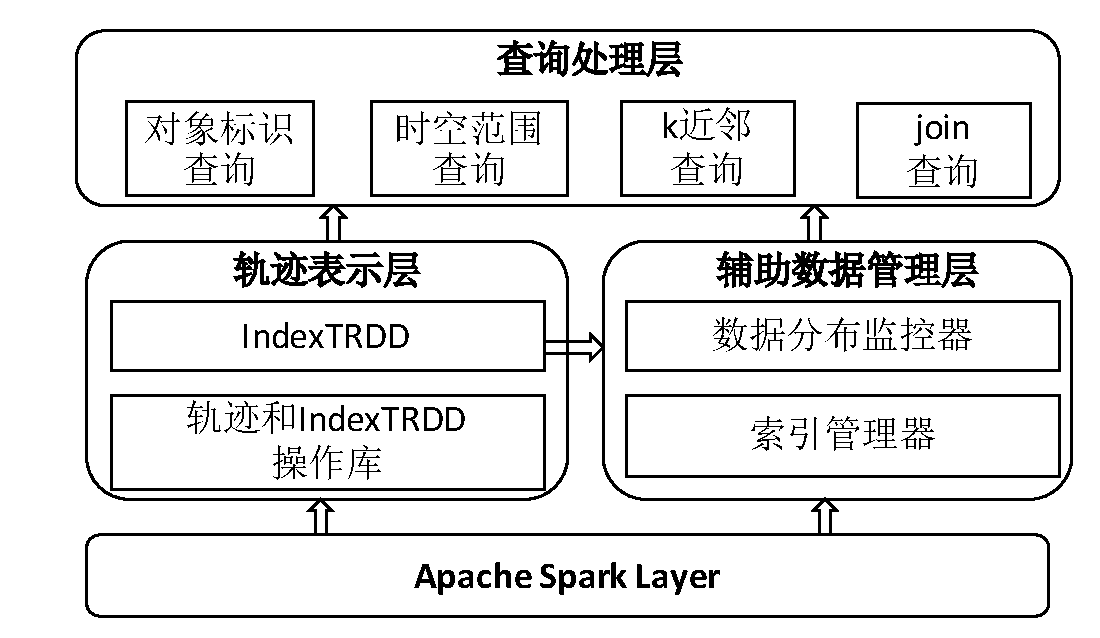
\includegraphics[width=0.73\textwidth]{Fig/chapter3/overview}
	\caption{剪枝示例}
	\label{fig-chapter3-architecture}
\end{figure}

TrajSpark系统架构如图\ref{fig-chapter3-architecture}所示,其由如下四层构成: (1)Apache Spark层,该层由Apache Spark提供的RDD及其常用操作构成;(2)轨迹数据表示层,该层介绍了对轨迹数据的抽象表示结构IndexTRDD;(3)辅助数据层,该层监控管理数据添加导致的数据分布变化,并负责指导对新数据的划分;(4)查询处理层,该层对三种典型轨迹查询进行了算法设计。具体地:

\begin{itemize}
	\item \textbf{Apache Spark 层:}  
	该层是整个系统的基础,其继承自Apache Spark,故不作详细介绍。
	
	\item \textbf{数据表示层:} 在该层,我们首先为轨迹设计了结合列存储形式的轨迹表示方法以达到压缩数据的目的。在TrajSpark系统中,轨迹以轨迹片段的形式存储,一条长轨迹将被切分成多条轨迹片段,而时空相邻的轨迹片段将被放到同样的数据分区中。
	为此,我们设计了基于轨迹片段的数据表示结构IndexTRDD,并提供了丰富的轨迹查询算子。为提高轨迹查询效率,TrajSpark为IndexTRDD维护了全局和局部两层轨迹索引。其中全局索引维护了所有分区的时空信息,而局部索引维护了每个分区内部轨迹的信息。该层是整个系统的核心。
	
	\item \textbf{辅助数据层:} 这一层维护了两种系统的全局信息。第一种就是轨迹数据的分布信息,其由数据分布监控器(Data Distributor Monitor)管理。随着数据不断装载入系统中,数据的分布会随之发生变化。TrajSpark通过监控这一变化并设计合理的数据划分方式以达到数据均衡的目的。第二种就是全局索引,其由索引管理者(Index Manager)维护。索引管理者运行在主节点上,用以管理数据的全局索引。当数据加载进后,索引管理这将更新全局索引。
	
	\item \textbf{查询处理层:} 这一层主要实现了两类基本轨迹查询以及轨迹$k$近邻查询。此外,用户可以通过基本函数接口实现更加复杂的查询。
\end{itemize}

\subsection{数据表示层}

\textbf{轨迹片段表示}
	
	原始来自轨迹GPS日志中的轨迹数据往往以轨迹点集的形式保存。因而,原始信息可以看作包含如下属性的表格$(MOID$, $Location$, $Time$, $A_{1}$, $\cdots$, $A_{n})$。其中$MOID$是移动对象的标识,  $Time$记录了轨迹点采集的时间、 $Location$代表轨迹点的位置。其他属性根据数据源的不同而变化。基于Spark的一个简单轨迹数据管理实现方案就是将轨迹数据看作由轨迹点构成的RDD。但该方案会导致数据的冗余,比如一个移动对象出现100次,则其标识将会重复100次。还有当连续采集的过程中,移动对象位置没有发生变化时,该位置仍然会被保存多次。
	除了数据冗余外,文献\cite{ChakkaEP03}表明基于轨迹片段的表示方式相比基于点的方式能显著提高查询效率。
	
	TrajSpark采用基于轨迹片段的方式管理轨迹数据。其将时空相邻的轨迹点聚集到统一数据分区中。此时,一条长轨迹可能被分割成若干段并存储在不同的分区上。在每一个分区内部,可以使用基于列存储的数据表达方式并结合数据压缩手段。实现这一目的存在两点挑战:
	(1)如何为非结构化的轨迹数据设计列存储的数据结构;(2)如何对列存储的轨迹数据进行压缩且不损害数据查询的效率。
	\begin{figure}
		\centering
		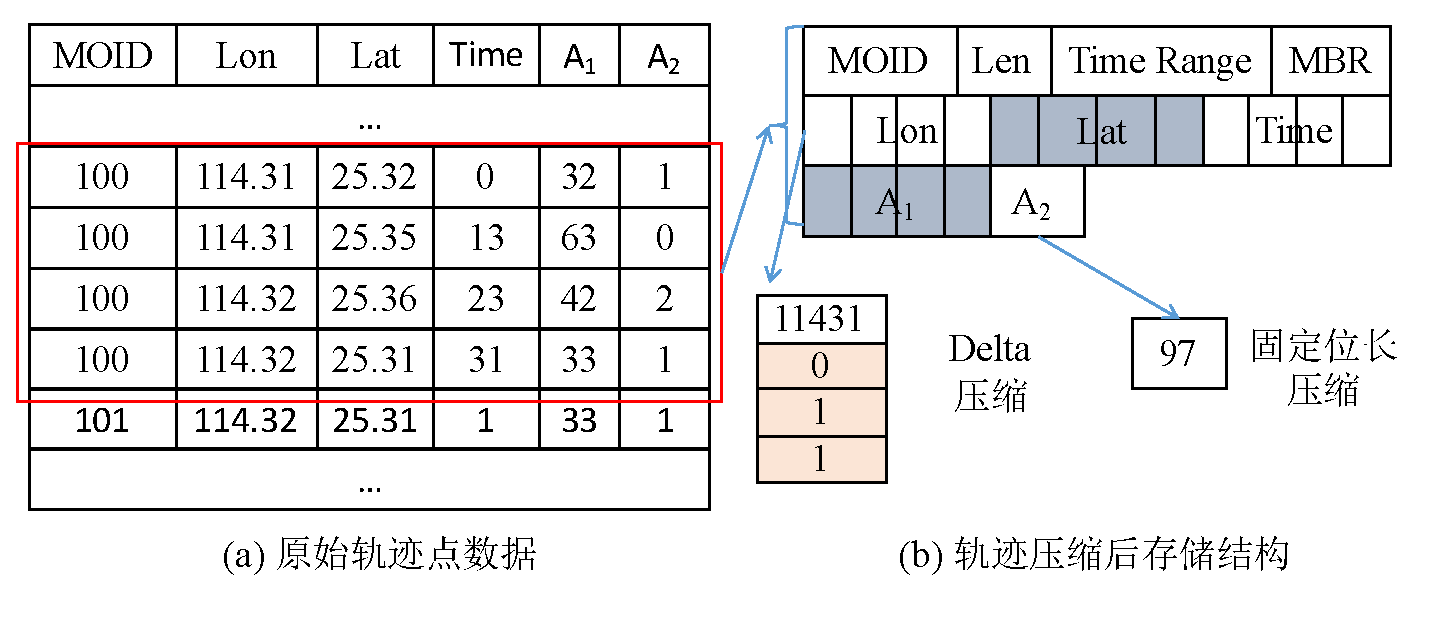
\includegraphics[width=0.95\textwidth]{Fig/chapter3/compress.eps}
		\caption{轨迹片段表示}
		\label{fig:TrajFormat}
	\end{figure}
	
	TrajSpark的实现方法是:在每一个分区内,先将所有轨迹点按照移动对象标识进行分组。接着属于同一移动对象的轨迹点按时间顺序进行排列,并得到一个轨迹片段。接着,将对每一个轨迹片段按
	图\ref{fig:TrajFormat}(b)所设计的表示方式进行压缩处理。在这种方式中,同一属性的值将被连续存放并压缩存储。其中针对数值型熟悉,如坐标位置等,使用差值压缩;对于枚举类型属性,使用固定为压缩。如图中$A_{2}$属性,其只有3个可能性的值即0、1和2。此时我们只需使用两个二进制位就能完成数据的存储。对于字符串属性,使用$gzip$进行压缩。压缩完所有数值后,我们为一条轨迹保留额外的概要数据,概要数据包含移动对象的标识、轨迹长度和(时空)最小包围盒信息。使用概要数据能对查询进行有效剪枝。最终,分区内轨迹点被转换为压缩好的轨迹片段,并使得整个轨迹数据集成为以轨迹片段构成的RDD(称之为TRDD)。
	
\textbf{轨迹片段索引}
	
	\begin{figure}[t]
		\centering
		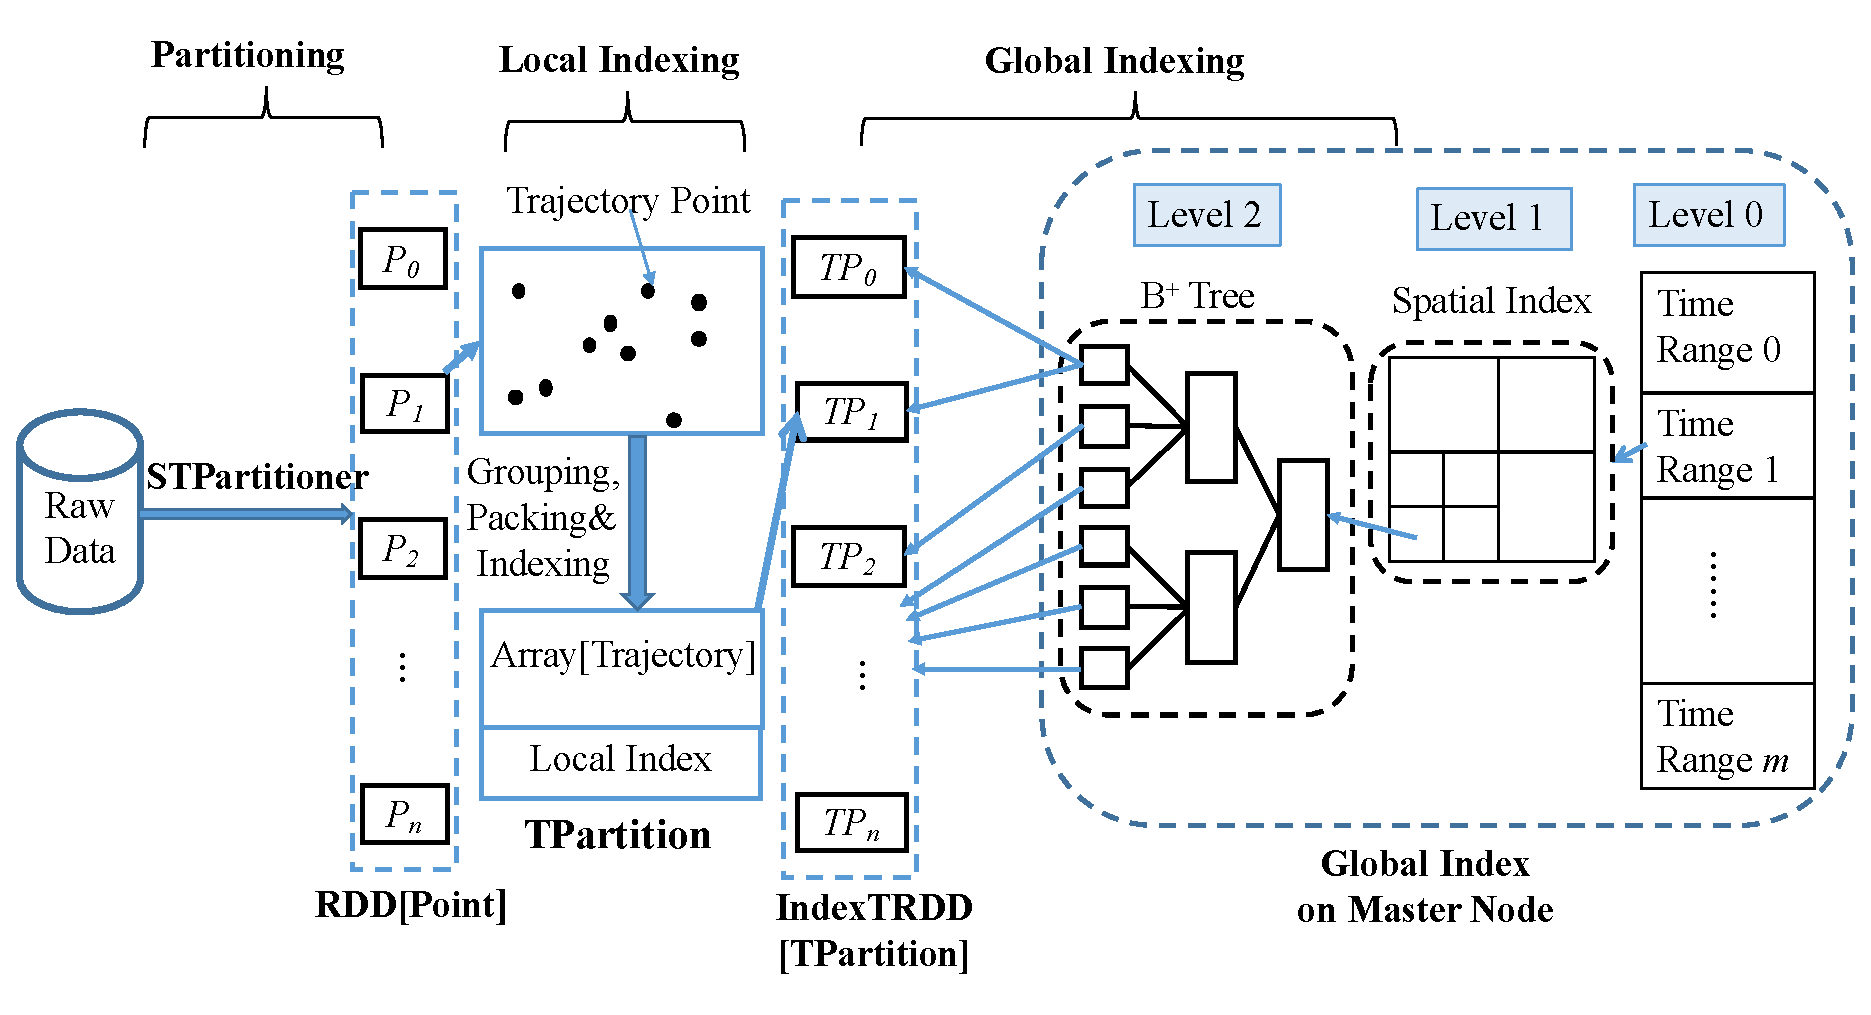
\includegraphics[width=0.95\textwidth]{Fig/chapter3/indexConstruct.eps}
		\caption{轨迹索引构建}
		\label{fig:index}
	\end{figure}
	
	前面,我们介绍了如何将原始的GPS记录转换成基于轨迹片段的TRDD。但TRDD对于给定的任意查询需要遍历整个数据集才能找到结果,因而CPU开销较大。为此,我们需要引入索引结构以提高查询效率。TrajSpark提出了IndexTRDD这一结构以支持索引。IndexTRDD首先通过在TRDD每个分区内引入针对轨迹标识的局部哈希索引,从而使得针对给定轨迹的查询复杂度降为常数级。进一步地,我们在IndexTRDD的分区之上构建了全局索引,以便查询执行时对不必要的数据分区进行剪枝。图\ref{fig:index}介绍了构建索引的整个数据流程,其包含:\emph{数据划分(Partitioning)}, \emph{局部索引构建(Local Indexing)}和\emph{全局索引构建(Global Indexing)}三个阶段。接下来将对这三阶段进行详细介绍。
	
	\emph{数据划分:}该阶段,TrajSpark将原始轨迹日志数据从磁盘装载进入磁盘形成一包含轨迹点对象的RDD。接着,我们需要对其进行数据划分以达到如下效果:(1)\textsf{数据局部性},即时空相邻的轨迹点需要划分到同一个数据分区中;(2)\textsf{负载均衡},各数据分区的数据量尽量相等;(3)\textsf{分区大小约束},每个分区数据大小要适中,以避免内存过载。尽管Spark本身提供了范围和哈希两种数据划分方法,但它们都是针对一维的数据进行划分。而轨迹是多维数据,这两种方式无法简单应用到轨迹划分中。为此,我们设计了新的针对轨迹的划分方法STPartitioner,该方法首先使用一颗四叉树或kd树来划分轨迹点。该索引树从原始轨迹的空间分布学习出来,以保证树的叶子节点所包含的轨迹点数量比较接近。当索引树构建好后,STPartitioner使用叶节点的边界进行数据划分。划分后,同一时空范围内的点被聚集到一起。
	为了保证每个分区大小适中,TrajSpark将聚集在一起的轨迹点根据移动对象标识或时间划分成若干大小相近的数据分区。
	
	\emph{局部索引构建:}经过数据划分后,轨迹数据集可看作是一个按时空划分好的点对象构成的RDD。在本阶段,我们首先将此RDD经过分组、排序和包裹以构建成以轨迹片段组织的TRDD。接着,为每个数据分区的头部添加一个局部哈希索引,用于将移动对象标识跟对应的轨迹片段映射起来。我们将这种包含索引及轨迹片段的分区称为TPartition。此时,整个数据集可看作由TPartition构成的RDD。我们称此时的RDD为IndexTRDD。最后,主节点收集每个分区的标识(每个数据分区都有一个特别的标识符)、分区所含数据的空间范围和时间范围等信息以便构建全局索引。
	
	\emph{全局索引构建:}本阶段,根据收集到的分区信息在主节点构建全局索引。全局索引的格式如图\ref{fig:index}所示,是一个三层混合索引。数据首先根据其时间维度信息被第0层粗粒度时间范围所划分。同时,每个粗粒度时间范围对应着一个第1维空间索引(STPartitioner就是根据这个空间索引对该时间范围内数据进行空间划分)。每个叶子节点所对应的空间范围可能包含若干数据分区,我们使用第2层B+树索引对这些分区根据时间维度进行管理。当第一批数据加载入系统后,第0层索引只包含一个时间值(时间段的起始时间),第1层空间索引即为数据划分所用的索引。我们收集每个分区的时间和空间信息以构建第2层索引。TrajSpark将全局索引保存在主节点的内存中并维护该索引的更新。即使当轨迹数据量很大时,我们的全局索引仍然只需消耗较少的存储空间,因而能以较低的内存开销放在主节点上。

\subsection{辅助数据层}

\textbf{数据分布管理器}

在真实的应用场景中,轨迹数据集会随着数据周期性的加载而不断变大\cite{AlyMHAOEQ15},从而导致数据的空间分布也发生变化。如何对新来的数据进行有效划分成为新的难点。一方面如果始终使用一个静态数据划分方式来划分,这样划分的开销虽低,但会导致数据不均衡从而影响查询的效率。另一方面,如果将新来的和已有的数据一起重新划分以得到均衡的结果(方法被文献\cite{SpatialSpark,Locationspark,GeoSpark,Simba}采用),但这样的划分开销太大(主要在数据Shuffle上)。并且重新划分已有的数据没有太大的必要,因为新数据的价值总是大于旧数据的,且用户的查询往往也是集中在新数据上。
所以当一批新数据到来时,TrajSpark尝试只均衡划分新数据而不改变已有数据的划分。这一点与AQWA 系统\cite{AlyMHAOEQ15}(需要对新的和已有的数据进行划分)有所区别。此外,TrajSpark只关注长时间段内的数据分布的变化,而尽量减轻短时间内数据分布的变化对数据划分的影响。比如周末与平时城市的轨迹分布会大不相同,但我们不应该应该这样的不同而对数据划分作太大变化。

基于以上考虑,数据分布管理器(Data Distribuion Monitor) 采用了时间衰减模型来监控数据分布的变化。该模型中给新来的数据更高的权重。具体做法是:首先,将整个空间维度划分成$m*m$个细粒度的格子,统计数每个格子内轨迹点的个数。当一批新数据到达时,数据分布管理器维护了两个矩阵:$A_{existing}$ 和 $A_{new}$, 用以分别记录已加载和新到达数据的分布。其中$A_{new}$为新数据在每个格子内点的个数除以总的点的个数得到。
当新数据达到后,$A_{existing}$通过将其每个值除以$\gamma$($\gamma$称为衰减因子,其给已有数据更低的权重)以降低自身的权重。然后,$A_{new}$加入到 $A_{existing}$ 中,并将其值赋为0。 因此,每当新数据加入后, 早期加入的数据权重会不断降低。为了更好的描述 $A_{existing}$的变化过程,我们使用$A_{existing}^{n}$来表示当地$n$次数据加入后数据的分布。

为自适应的调整数据划分策略,我们使用矩阵$PA_{c}$来描述当前划分方式所依赖的数据分布,其用$A_{existing}^{0}$来初始化。
STPartitioner就是从$PA_{c}$中学习出数据划分的索引并将数据按照空间维度进行划分。当第$n$批数据到达后,$PA_{c}$与$A_{existing}^{n}$ 的分布差别超过一个给定的阈值,则认为数据发生了较大变化。此时,需要更新数据划分策略。我们的做法是将 $A_{existing}^{n}$的值赋予给$PA_{c}$, 并从$PA_{c}$中学出新的索引用以替换STPartitioner中用于数据划分的索引。在TrajSpark,我们使用JSD距离来度量两个分布的差别(两个分布均需归一化后才能计算)。本文使用的时间窗口衰减模型具有延迟更新特性,能很好的应对数据短时间内发生较大变化的情况。

\textbf{索引管理器}

索引管理器(Index Manager)主要维护索引的更新和持久化。在Spark中存在着两种情况会导致全局索引的变化。第一种情况是当STPartitioner更新了其用于数据划分的空间索引。在这种情况下,我们会在全局索引的第0层的最后添加新的时间范围起点,同时为该范围添加对应的第1层空间索引。第二种情况是当新到达数据的所有分区加入到IndexTRDD中后,这些分区所对应的信息也会被添加到全局索引中。
索引管理器将全局索引存储在主节点内存上。此外,它可以选择将索引持久化到文件系统中也能将其再次从文件读入到内存中。这使得系统能够在出现异常下进行快速恢复。值得注意的是,TrajSpark对全局索引提供了一系列的操作接口,如交集运算(intersect)、范围覆盖计算(overlap)等,以满足用户对全局索引的操作需求。

\subsection{查询处理层}
在这一层,我们将介绍TrajSpark如何处理三种典型的轨迹查:基于给定对象标识的查询、时空范围查询以及$k$近邻查询。

\textbf{基于对象标识的查询}

\begin{algorithm}[t]    %算法的开始
	\setlength{\abovedisplayskip}{8pt}
	\setlength{\belowdisplayskip}{8pt}
	\caption{基于对象标识的查询算法}   %算法的标题	 
	\label{alg:so}       %给算法一个标签,这样方便在文中对算法的引用
	\begin{algorithmic}[1] 
		\REQUIRE $moid$, $tRange$;
		\ENSURE one trajectory;
		\STATE $pids$ = gIndex.intersect($tRange$);
		\STATE $ts$ = IndexTRDD.PartitionPruningRDD($pids$)\\
		\qquad \qquad \qquad \qquad .getTraWithID($moid$).mapValues(sub($tRange$));
		\RETURN 	  $ts$.reduceByKey(merge).collect();
	\end{algorithmic}
\end{algorithm}	 

基于给定对象的查询通过接收待查询轨迹的标识$moid$和时间约束范围$tRange$,以返回该移动对象在指定时间范围内的轨迹。尽管Spark可以通过最基本的filter 算子实现查找,但该方式需要遍历整个数据集,因而CPU开销较高。TrajSpark通过使用内部两层索引机制能进行快速的剪枝。其处理方法基于以下三点观察:(1)全局索引的第0层能够快速剪枝掉不满足时间约束的分区,并且第2层时间范围索引能够快速找出与给定时间范围相交的分区;(2)对于每个数据分区,可以通过局部的哈希索引快速找出指定移动对象的轨迹;(3)指定对象轨迹的概要数据包含时间范围,利用该范围可以快速判断,该移动对象在指定时间是否有数据。

基于以上观察,我们设计了查询算法\ref{alg:so}。TrajSpark首先遍历全局索引找出时间范围与给定时间约束相交的分区(第1行)。该操作可以通过全局索引的 intersect接口实现。接着,IndexTRDD 调用 Spark系统 API--- PartitionPruningRDD, 来找出这些分区内容。然后,TrajSpark通过局部索引找到给定移动对象的轨迹片段,并找出指定时间内的数据(第2行)。最后,汇总每个分区所找出的子轨迹片段,并合并成一条完整的轨迹(第3行)。TrajSpark提供了merge算子用于合并同一对象的两条轨迹并将结果按时间序排列。

	\textbf{时空范围查询}
	
\begin{algorithm}[h]    %算法的开始
	\caption{时空范围查询算法}   %算法的标题	 
	\label{alg:st}       %给算法一个标签,这样方便在文中对算法的引用
	\begin{algorithmic}[1] 
		\REQUIRE $tRange$, $sRange$;
		\ENSURE a set of trajectories;
		\STATE $pids$ = gIndex.intersect($tRange$, $sRange$);
		\STATE $ts$ = IndexTRDD.PartitionPruningRDD($pids$) \\
		\qquad \qquad \qquad \qquad .filter($tRange$, $sRange$) \\
		\qquad \qquad \qquad \qquad	.mapValues(sub($tRange$, $SRange$));
		\RETURN 	  $ts$.reduceByKey(merge).collect();
	\end{algorithmic}
\end{algorithm}

时空范围查询通过接收时间范围参数$tRange$和空间范围参数$sRange$返回指定时空范围内的轨迹。需要指出的是,这两个查询参数可以不全部给出。
通过使用索引,TrajSpark也能为该查询提供远胜于遍历操作的查询效果。算法\ref{alg:st} 介绍了该查询的实现方法。其首先通过全局索引找出与给定时空范围相交的分区(第1行)。接着,对每个分区内的轨迹通过访问其概要数据以剪枝掉与给定时间范围没有交集的轨迹片段。然后对满足约束的片段进一步找出满足时空约束的子片段(第2行)。最后,将满足时空范围内的子片段按照移动对象标识分组,同一个移动对象的子片段进行合并 得到完整的轨迹(第3行)。

\begin{algorithm}    %算法的开始
	\setlength{\abovedisplayskip}{8pt}
	\setlength{\belowdisplayskip}{8pt}
	\caption{$k$近邻查询算法}   %算法的标题	 
	\label{alg:knn}       %给算法一个标签,这样方便在文中对算法的引用
	\begin{algorithmic}[1] 
		\REQUIRE $IndexTRDD$, $disM$;
		\ENSURE the $k$ most similar trajectories to $tr$;
		\STATE $mbr = tr.MBR$, $tRange=tr.TimeRange$;
		\REPEAT
		\STATE $pids$ = gIndex.intersect($mbr$, $tRange$);
		\STATE $ts$ = IndexTRDD.PartitionPruningRDD($pids$)\\
		\qquad \qquad \qquad \qquad         .filter($mbr$, $tRange$) \\
		\qquad \qquad \qquad \qquad	.reduceBykey(merge);
		\STATE $mbr$.expand($1+\alpha$);
		\UNTIL{($ts$.size $>$ $k$)}
		\STATE $candidate$=$ts$.collect();
		\RETURN $candidate$.map($t\rightarrow $(distance($t,tr$),$t$))\\
		\qquad \qquad \qquad \qquad	.sortByKey.top($k$);
	\end{algorithmic}
\end{algorithm}


\textbf{$k$近邻查询}


$k$近邻轨迹查询,即给定查询轨迹,从轨迹数据集中找出与之距离最近的$k$条轨迹。该查询接受两个参数:一个是待查询轨迹$tr$,另一个是距离度量方式$distance$。
尽管轨迹距离度量准则有很多,但都遵循着时空范围越接近,则距离越近原则。为此设计了算法 \ref{alg:knn}以支持任一距离在$k$近邻查询的使用。首先 TrajSpark获得待查询轨迹的空间包围信封和时间范围(第1行)。接着,利用全局索引,找出与查询时空范围相交的分区,然后在每个分区内找出与轨迹时空范围相临交的轨迹片段,并将这些片段按照标识和时间拼接成完整的轨迹 (第2行)。此时,需要检查拼接后的轨迹数目是否有$k$个,如果不足$k$个,则进一步扩大搜索空间,直到找到超过$k$个为止。其中扩大搜索空间的方法是将搜索范围的长度和宽度同时变为原来的$1+\alpha$ ($0 < \alpha < 1$)倍。
最后,对搜集到的轨迹进行真实距离计算,并找出距离最近的$k$条。

\textbf{Join查询}

 \begin{figure}[t]
	\centering
	\subfigure[]{  
		\label{fig:maptoEntry}
		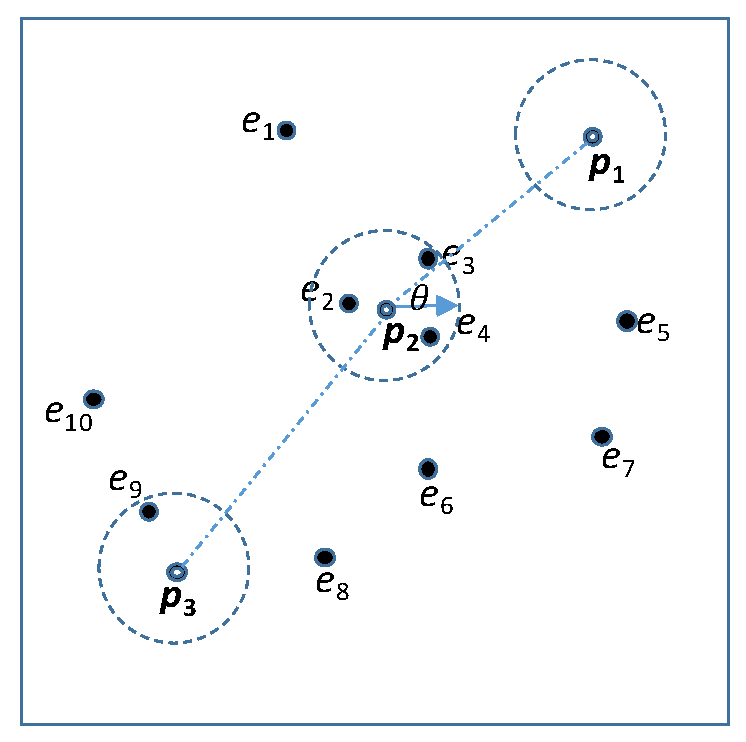
\includegraphics[width=2.7in]{Fig/chapter3/joinmap.eps}	
	}
	\subfigure[]{
		\label{fig:gridindex}
		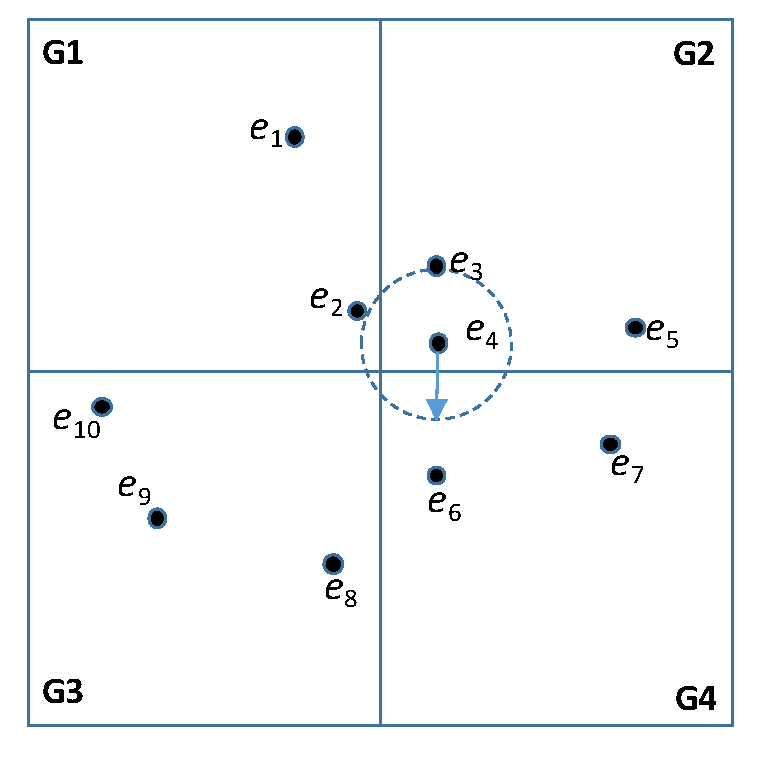
\includegraphics[width=2.7in]{Fig/chapter3/quadtree.eps}
	}
	\subfigure[]{
		\label{fig:globaljoin}
		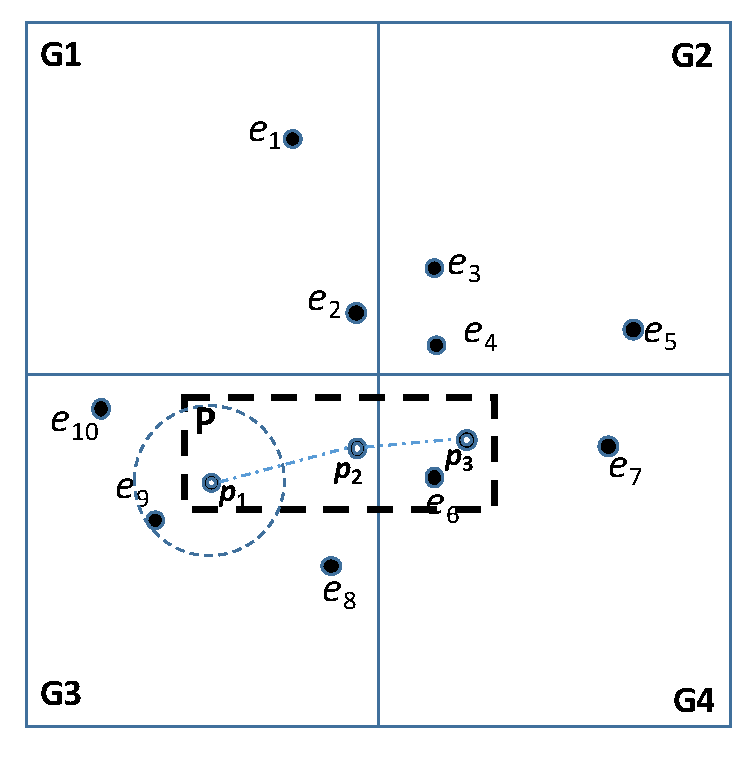
\includegraphics[width=2.7in]{Fig/chapter3/globaljoin.eps}
	}
	\caption{Join查询示例}
	\label{fig:joinprepare}
	\vspace{-0.5cm}
\end{figure}
轨迹的join查询被广泛应用在社交网络和推荐系统中。一个典型的查询应用就是,给定一个轨迹数据集和一个带语义信息的空间对象集合(如POIs、道路和区域),研究者们将这两个数据集关联起来以得到语义轨迹。这样的一个查询可表示为\textbf{Join($IndexTRDD, SP,\epsilon$)},其中 $IndexTRDD$代表轨迹数据,$SP$ 代表空间对象数据集,$\epsilon$ 是查询的空间约束。这个查询将轨迹中的点$p$映射到$SP$中距离最近的点$e$上,且需满足$p$到$e$的距离需小于$\epsilon$。如果点$p$找不到满足条件的映射点,则会将其忽略。图\ref{fig:joinprepare}给出了查询示例,给定查询轨迹$< p_{1}, p_{2}, p_{3}>$ 和由10个点对象构成的空间对象集合(由$e_{1} $ 到 $e_{10}$表示)。根据查询,$p_{1}$ 不会被映射到任何点上, $p_{2}$会被映射到 $e_{2}$ 上,因为 $e_{2}$是$\epsilon$ 范围内最近的点,  $p_{3}$ 将会被映射到 $e_{9}$ 上。

由于轨迹数据集和空间数据集都比较大,暴力查找开销较高。为此,我们需要对$SP$数据集进行预处理。由于整个系统空间被划分成了$m*m$个格子,我们首先对$SP$数据集统计每个格子里点的个数。假设$SP$将被划分成$S$个分区(每个分区对应一个网格,且$S$值由$SP$和分区大小约束两方面决定)。然后,我们构建四叉树或R树来构建索引管理这些格子,使得最终索引树的叶子节点为$S$个。接着,用构建好的树索引划分$SP$得到一个 PairRDD,PairRDD的每个元素的value值为对应的空间点,key值为与该点$\epsilon$范围相交的网格标识。由于点的$\epsilon$范围可能与多个网格相交,因此一个点可能会形成多个键值对。
Fig. \ref{fig:gridindex}介绍了当使用四叉树来划分$SP$时的案例。在该图中,点$e_{4}$ 被映射成4个键值对$<G1,e_{4}>, <G2, e_{4}>, <G3, e_{4}>, <G4, e_{4}>$。最后,我们对这样的PairRDD中键相同的元组看作为一个分区,并对该分区内部空间点构建局部索引。这样$SP$就被转换成具有局部和全局两层索引。完成以上对空间数据集的预处理后,我们设计了如下join查询算法,该算法包含三个主要步骤:全局join,局部join和合并。下面将对这三个部分进行详细介绍。

\textbf{全局 join.} 在该阶段,根据$IndexTRDD$和$SP$的全局索引,将两者有交集的分区形成分区对。如图\ref{fig:globaljoin}所示,带有虚线的方框$P$代表了$IndexTRDD$的一个分区的包围矩形。$P$跟$SP$数据集的$G3$ 和 $G4$相交,因此会形成两个新的数据分区$\langle P, G3\rangle$和$\langle P, G4\rangle$。其中$\langle P, G3\rangle$包含了IndexTRDD的$P$分区和$SP$的$G4$分区的数据。
其中由于$G3$和$G4$所代表的分区包含了除自身范围外还有其边界外$\epsilon$范围内的点(图中$e_4$存在于$G3$和$G4$所对应的分区中),所以构成的分区对会包含join查询结果的完备集。因此,我们对两个数据集的全局索引使用传统的空间join算法,得到相交的分区对。最终,将所有分区对的数据整合在一起,形成新的数据集。

\textbf{局部join.}根据上一步得到的结果,对每一个分区内的属于轨迹的那部分数据,逐步遍历每条轨迹,并对每个点从$SP$部分的索引中找出满足$\epsilon$ 约束的最近邻点。若每个轨迹点找到满足条件的点,则将原始轨迹的位置信息,替换为对应匹配点的信息。若找不到满足条件的点,则忽略该轨迹点。局部join产生的数据即为映射后的轨迹数据,只是将原来的位置信息维度替换为空间数据的标识。
由于某个空间点会存在多个分区中,因此局部匹配后的结果会出现对一个轨迹

 \textbf{合并.}由于$IndexTRDD$的一个分区会与$SP$的多个分区相交,所以存在着某个轨迹点在一个$SP$分区中没有匹配点,但在另一个$SP$分区中有匹配点的情况。如图 \ref{fig:globaljoin}中, $<p_{1}, p_{2}, p_{3}>$ 是一段位于分区 $P$中的片段。当$P$ 和 $G4$产生分区对时,$p_{1}$将不会被匹配到任何点,但是当$P$ 和$G3$构成的分区对时, $p_{1}$会被匹配到$e_{9}$上。因此,在该阶段,我们需要对局部join的结果进行合并以形成最终的结果集。


\section{实验分析}\label{sec-c3-exp}

\subsection{实验设置}
\begin{table}[t]
	\centering  
	\renewcommand\arraystretch{1.2}
	\begin{tabular}{|c|c|c|c|} 
		\hline
		数据集 & 时间 & 记录数 & 大小(Gb)  \\ \hline
		真实数据集 & 2013.10.1-12.31 & 约250万 & 190  \\ \hline
		人工数据集 & 2013.10.1-12.31& 约 1.8亿 & 1400\\ \hline
	\end{tabular}
	\caption{TrajSpark数据集描述}
	\label{table:SystemData}
\end{table}
在本章节我们将验证系统的性能。所有的实验是在由12个节点构建的分布式集群上实现。每个节点包含一个8核Intel E5335 2.0GHz处理器和16G内存,每个节点的操作系统为Ubuntu 12.0.4,并运行着Spark 1.5.2。Spark集群以standalone模式部署。



我们使用了两个轨迹数据集来验证系统的性能\cite{TrajSpark},包含一个真实轨迹数据集合一个人工合成的轨迹数据集。数据集描述如
表\ref{table:SystemData}所示,这两个数据集为13,007量北京出租车在3个月内(2013年10月至12月)产生的轨迹数据。每条记录包含了如下信息:车的标识、采集时间、经度、纬度、速度和角度等其他描述信息。真实数据集含约250万条轨迹日志记录,数据量为190Gb。为了更好的演示TrajSpark系统的可扩展性,我们根据真实数据集生成了人工数据集。生成方法为将出租车在运行过程中的点通过差值法增加数据使得每5秒种有一个点产生。生成的人工数据集含约1.8亿条记录,数据量为1.4Tb。需要指出的是,真实数据集可以完全被加载入系统内存,而人工数据集无法被完全加载。

在TrajSpark系统中我们将整个北京空间划分成$1,000*1,000$个细格子,使得每个格子覆盖的范围为180m*180m。我们将TrajSpark跟最新的两个空间数据管理系统GeoSpark和Simba从查询延迟和可扩展性两方面进行对比分析。其中延时指标使用10个查询的平均时间进行计算。


\subsection{实验结果及分析}

	\begin{figure}[t]
	\centering
	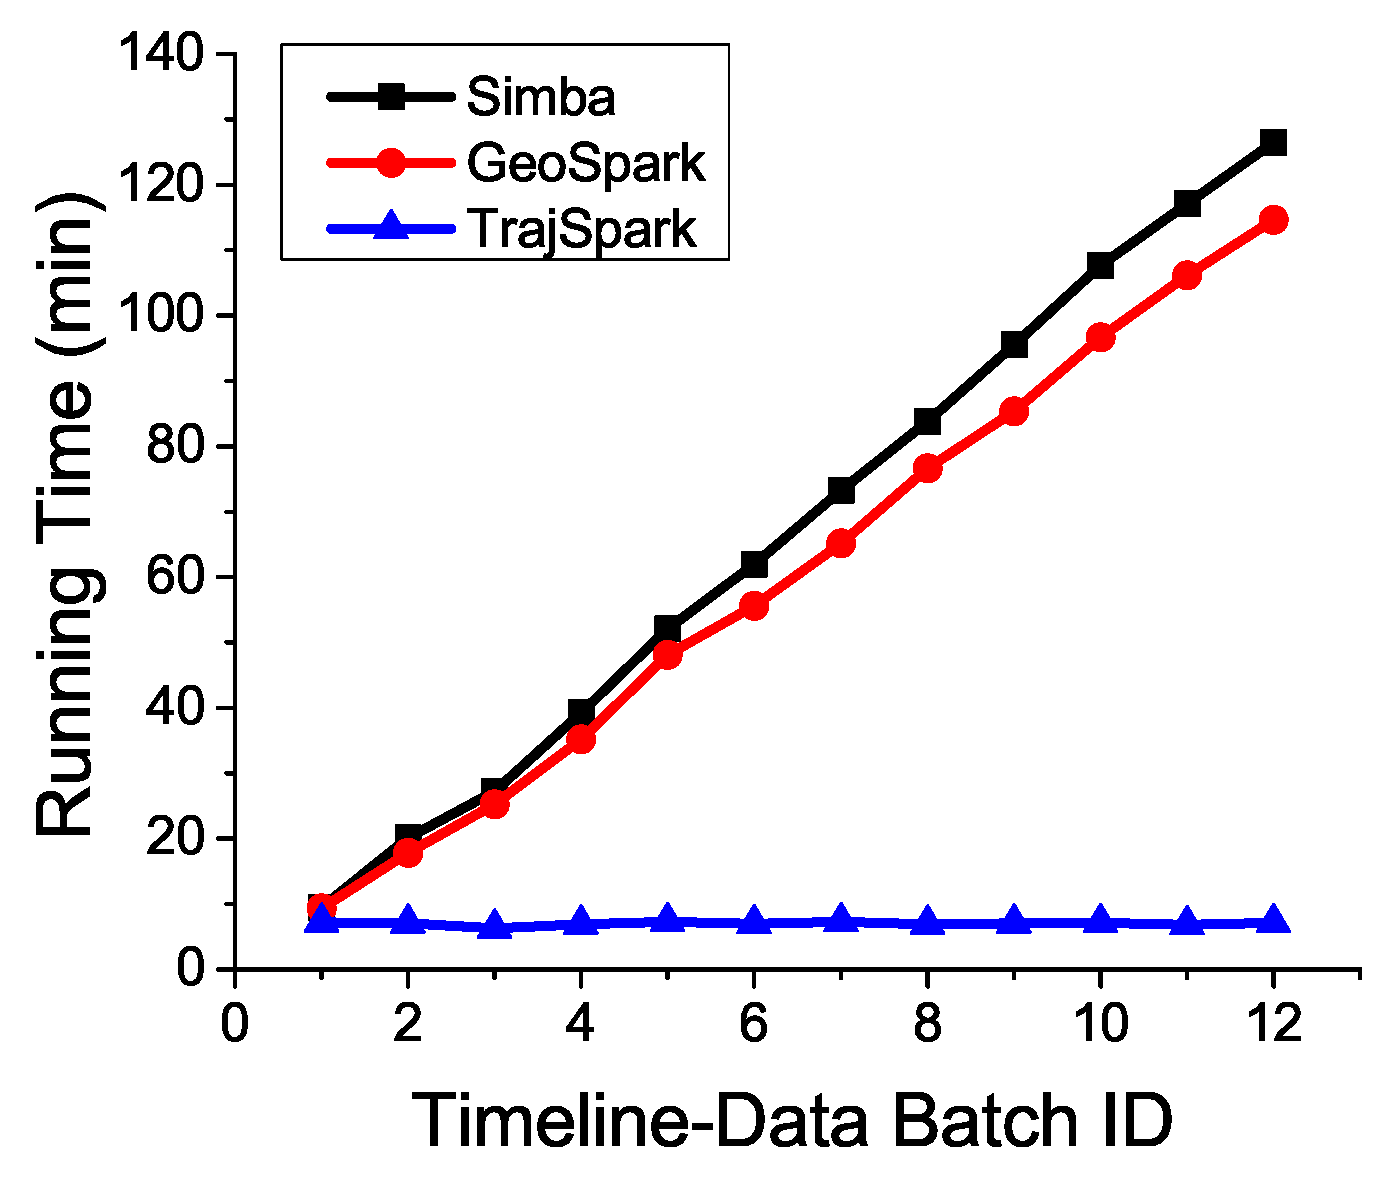
\includegraphics[width=3in]{Fig/chapter3/loadfinal.eps}
	\caption{数据加载开销}
	\label{fig:loadtime}
\end{figure}

首先,我们研究了系统加载数据的时间开销。图\ref{fig:loadtime}介绍了当所有系统随着数据不断导入到系统,系统更新一批数据的时间开销,其中每一批数据的大小为32Gb。
从图中可以发现GeoSpark和Simba都随着已转入数据量的增加导致新来的数据加载时间呈线性增加。这是由于这两个系统会将已有数据和新来的数据结合起来统一考虑,然后将两者作为整体重新划分。划分的过程会导致数据的洗牌,占用较多的网络通信和磁盘I/O开销。而TrajSpark由于只需对新来的数据进行数据划分,然后将划分后的分区信息汇总入全局索引中。因此,划分开销并不会随着数据的增加而发生较大变化。综上所述,TrajSpark具有较好的数据可扩展特性。


 \begin{figure}[t]
	\centering
	\subfigure[RDD存储开销]{
		\label{fig:local}
		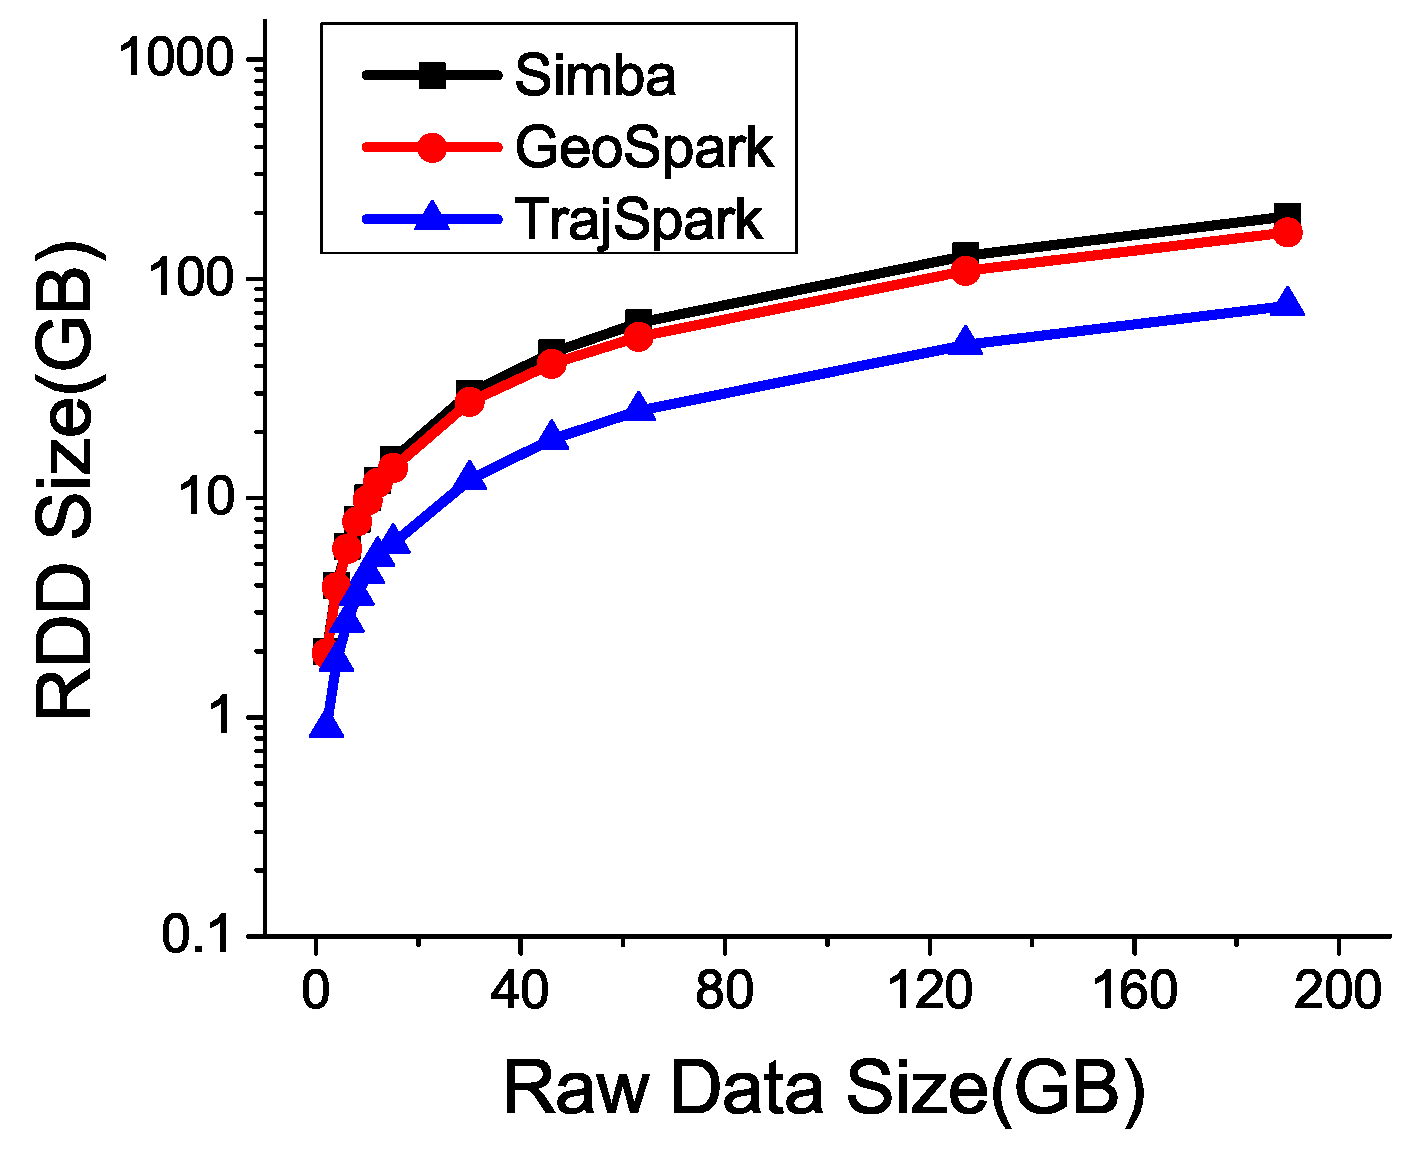
\includegraphics[width=2.7in]{Fig/chapter3/LI.eps}		
	}
	\subfigure[全局索引存储开销]{
		\label{fig:global}
		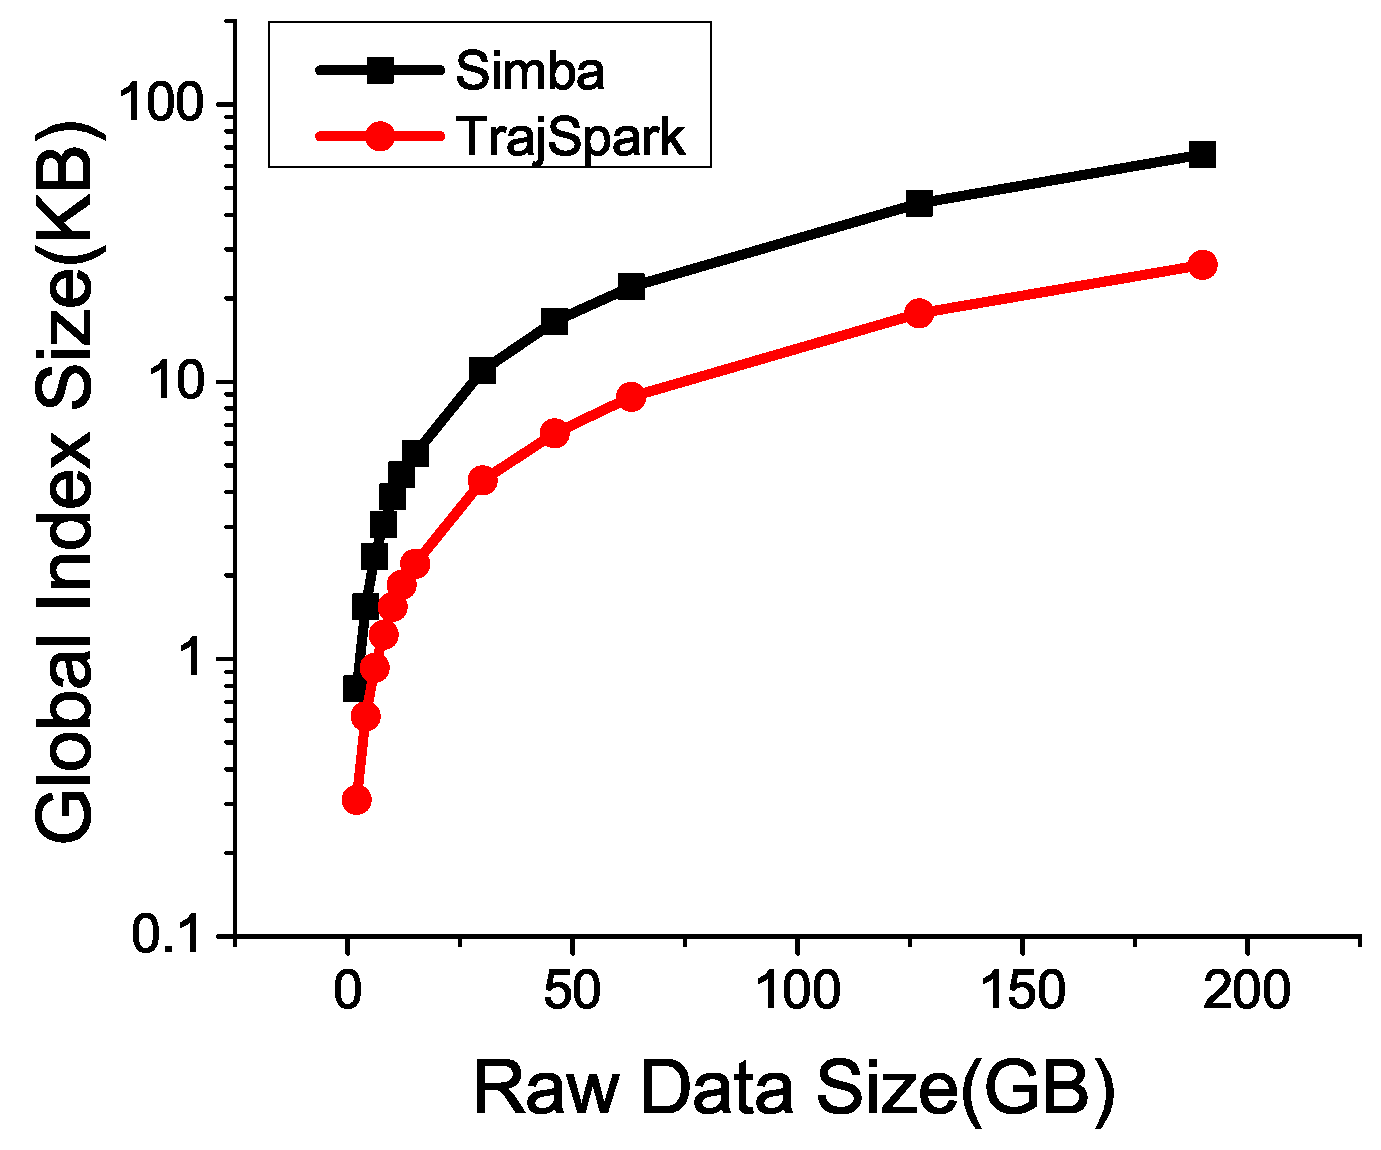
\includegraphics[width=2.7in]{Fig/chapter3/GI.eps}
	}
	\caption{数据存储开销}
	\label{fig:storage}
\end{figure}

接着,我们研究了从IndexTRDD和全局索引两部分的存储开销随数据量的变化情况。图\ref{fig:storage}展示了3个系统当不同数据量级的轨迹数据加载后,数据存储和全局索引两者存储开销的变化情况。其中图\ref{fig:local}显示当数据加载入TrajSpark系统后,所消耗的存储开销最低。而当加载入Simba和GeoSpark后消耗的存储开销是TrajSpark的2-3倍。这是因为TrajSpark会将原始轨迹数据按列存储形式存放并进行压缩,而后两者直接存放原始数据,数据冗余较多。图\ref{fig:global}介绍了3个系统的全局索引存储开销。从图中可以发现这一开销在三个系统内部均较少(数量级为Kb),因而都可以轻松存放到内存中。其中TrajSpark系统的全局索引开销最少(约是Simba的1/3),这是因为其数据压缩后,每个分区能放入跟多的数据,从而导致分区数较少。而全局索引是构建在分区之上的,所以TrajSpark会消耗更少的内存来存放全局索引。



然后,我们验证了TrajSpark在基于给定对象的查询在不同数据量下的效果。图\ref{fig:ID-based} 展示了查询性能。从该图中我们可以发现TrajSpark比Simba快了一个数量级,且比GeoSpark快了两个数量级。这是由于GeoSpark需要遍历整个数据集,所以其效果最慢。而Simba虽然能通过全局索引剪枝掉不相关的数据分区,但它仍然需要遍历每个分区内部的所有数据。相比较而言,TrajSpark既使用了全局索引剪枝分区,又在每个分区内使用局部哈希索引进行随机访问。
需要注意的是,这些系统在真实数据集上的延时比人工数据集下的低。这是由于内存容量可以存放大部分真实数据集,而只能转载的下少部分人工数据集。所以人工数据集下的查询会有额外的I/O开销。尽管如此,这些系统在人工数据集下仍取得较好的结果。这是由于以下两点原因:(1)我们将数据以``MEM\_AND\_DISK\_SER''形式存放,经常被访问的数据会被存放到内存中;(2)使用全局索引,能避免很多I/O开销。
\begin{figure}[t]
	\centering
	\subfigure[真实数据集]{  
		\label{fig:RealID}
		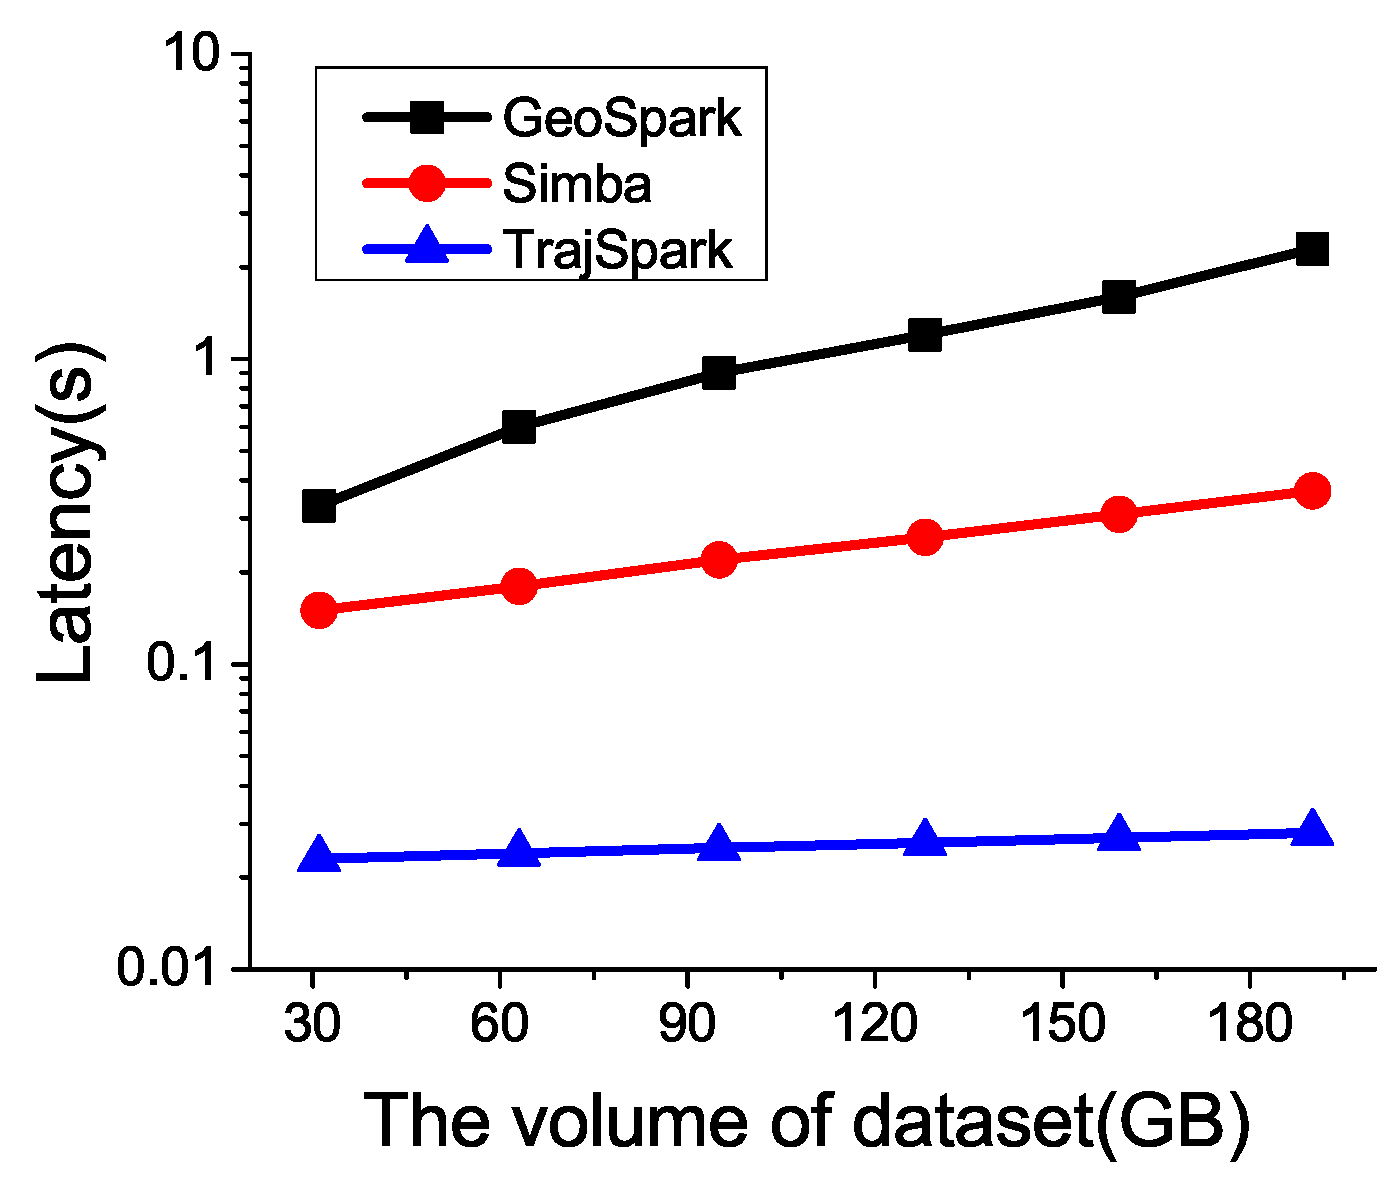
\includegraphics[width=2.7in]{Fig/chapter3/idS.eps}	
	}
	\subfigure[人工数据集]{
		\label{fig:synthetic}
		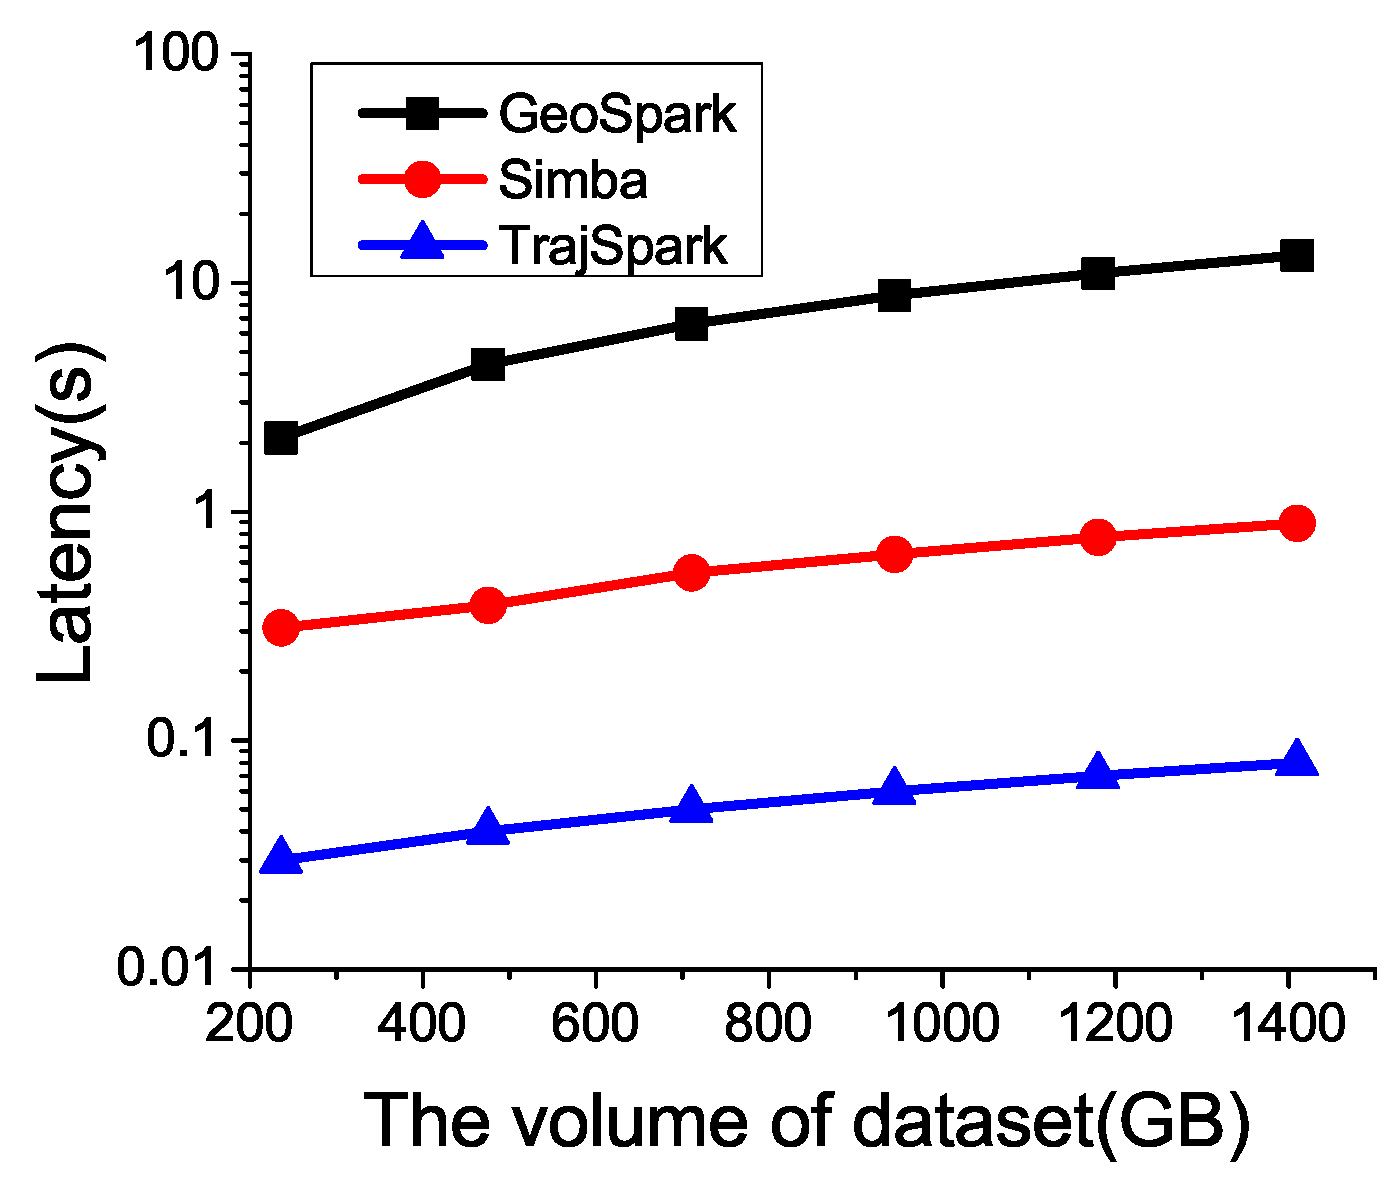
\includegraphics[width=2.7in]{Fig/chapter3/idB.eps}
	}
	\caption{基于给定对象的查询性能}
	\label{fig:ID-based}
\end{figure}

\begin{figure}[t]
	\centering
	\subfigure[真实数据集]{  
		\label{fig:RealST}
		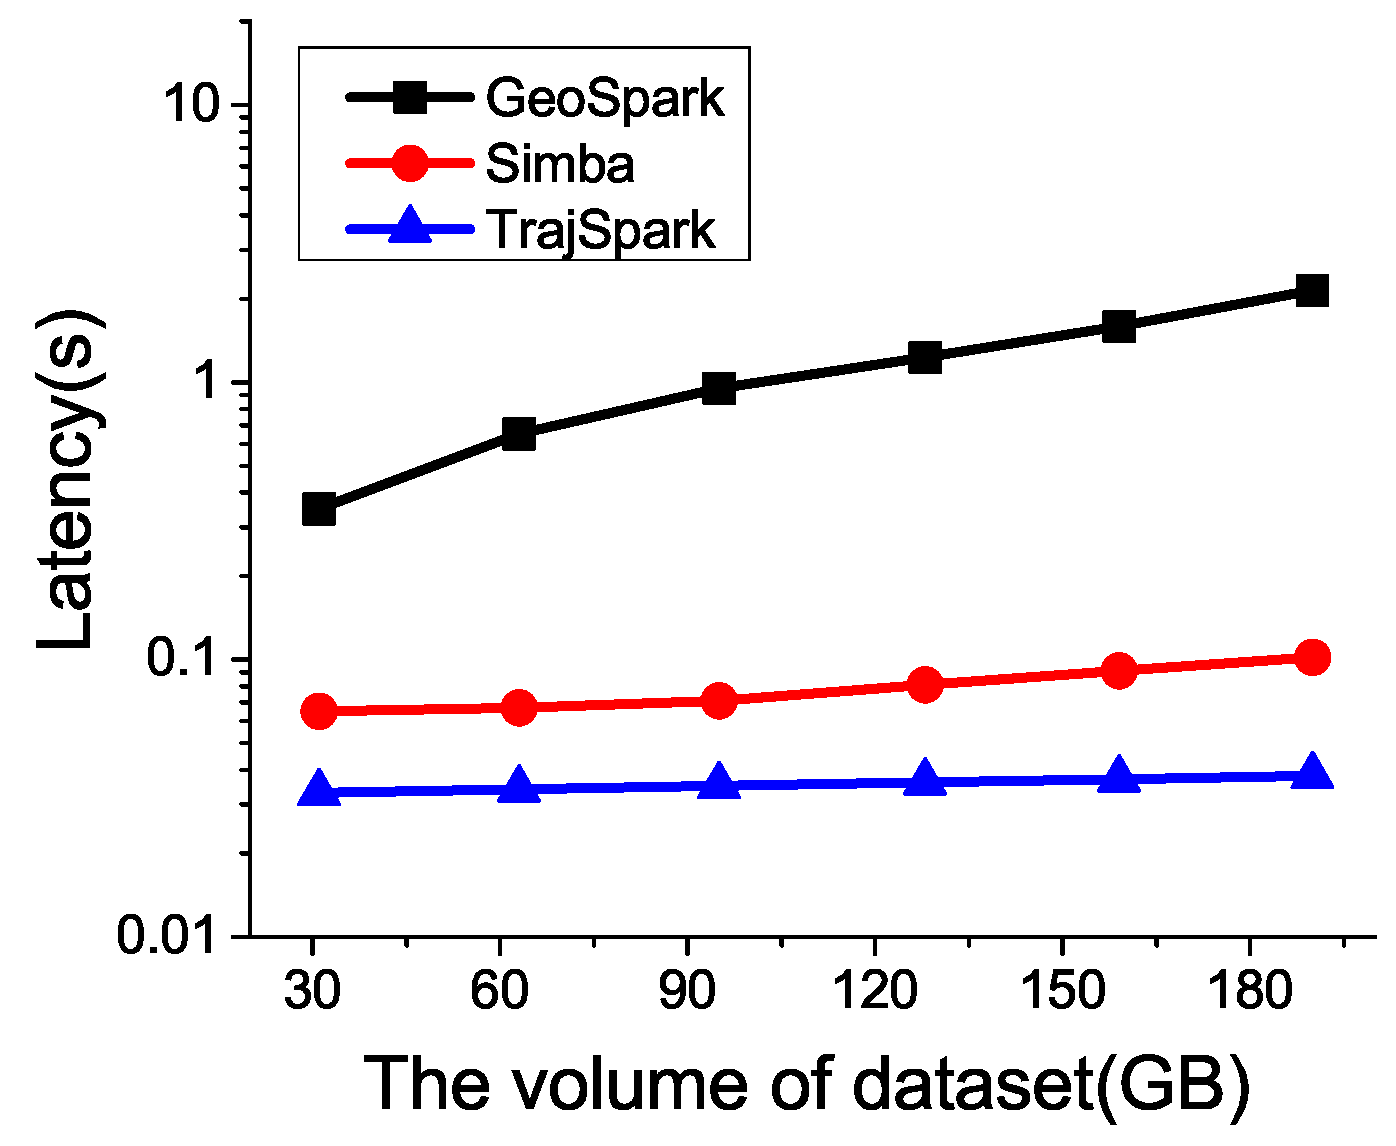
\includegraphics[width=2.7in]{Fig/chapter3/RangeS.eps}	
	}
	\subfigure[人工数据集]{
		\label{fig:syntheticST}
		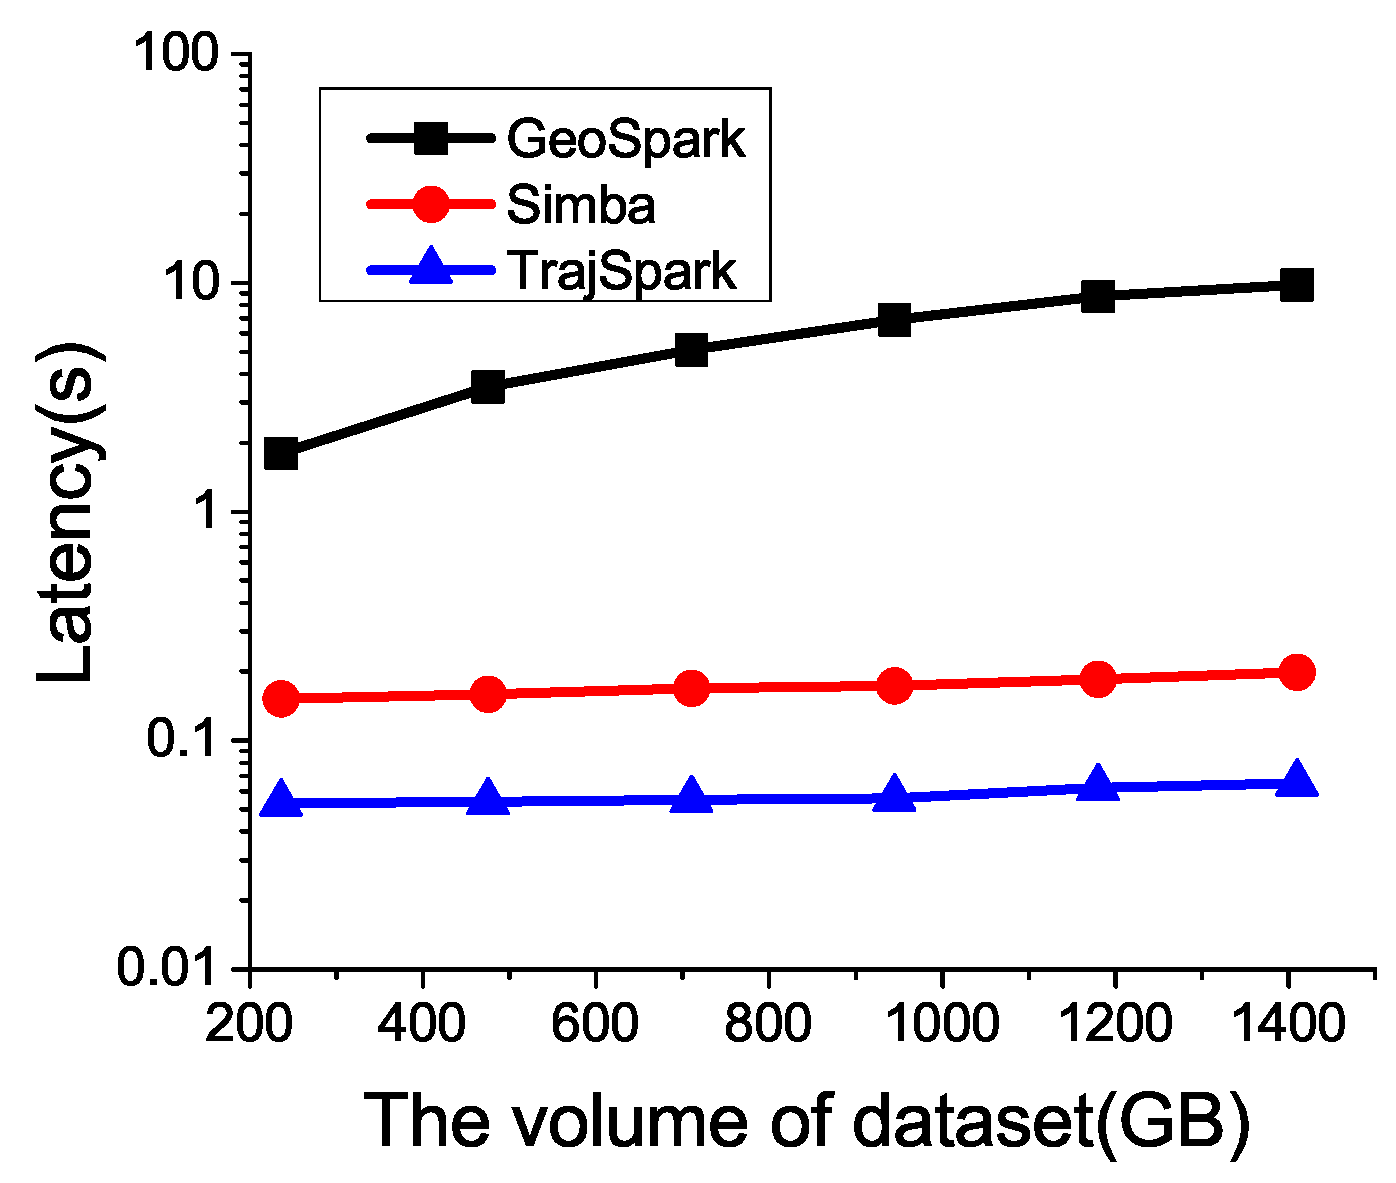
\includegraphics[width=2.7in]{Fig/chapter3/RangeB.eps}
	}\\
	\subfigure[TrajSpark---真实数据集]
	{  \label{fig:RealSPVarious}
		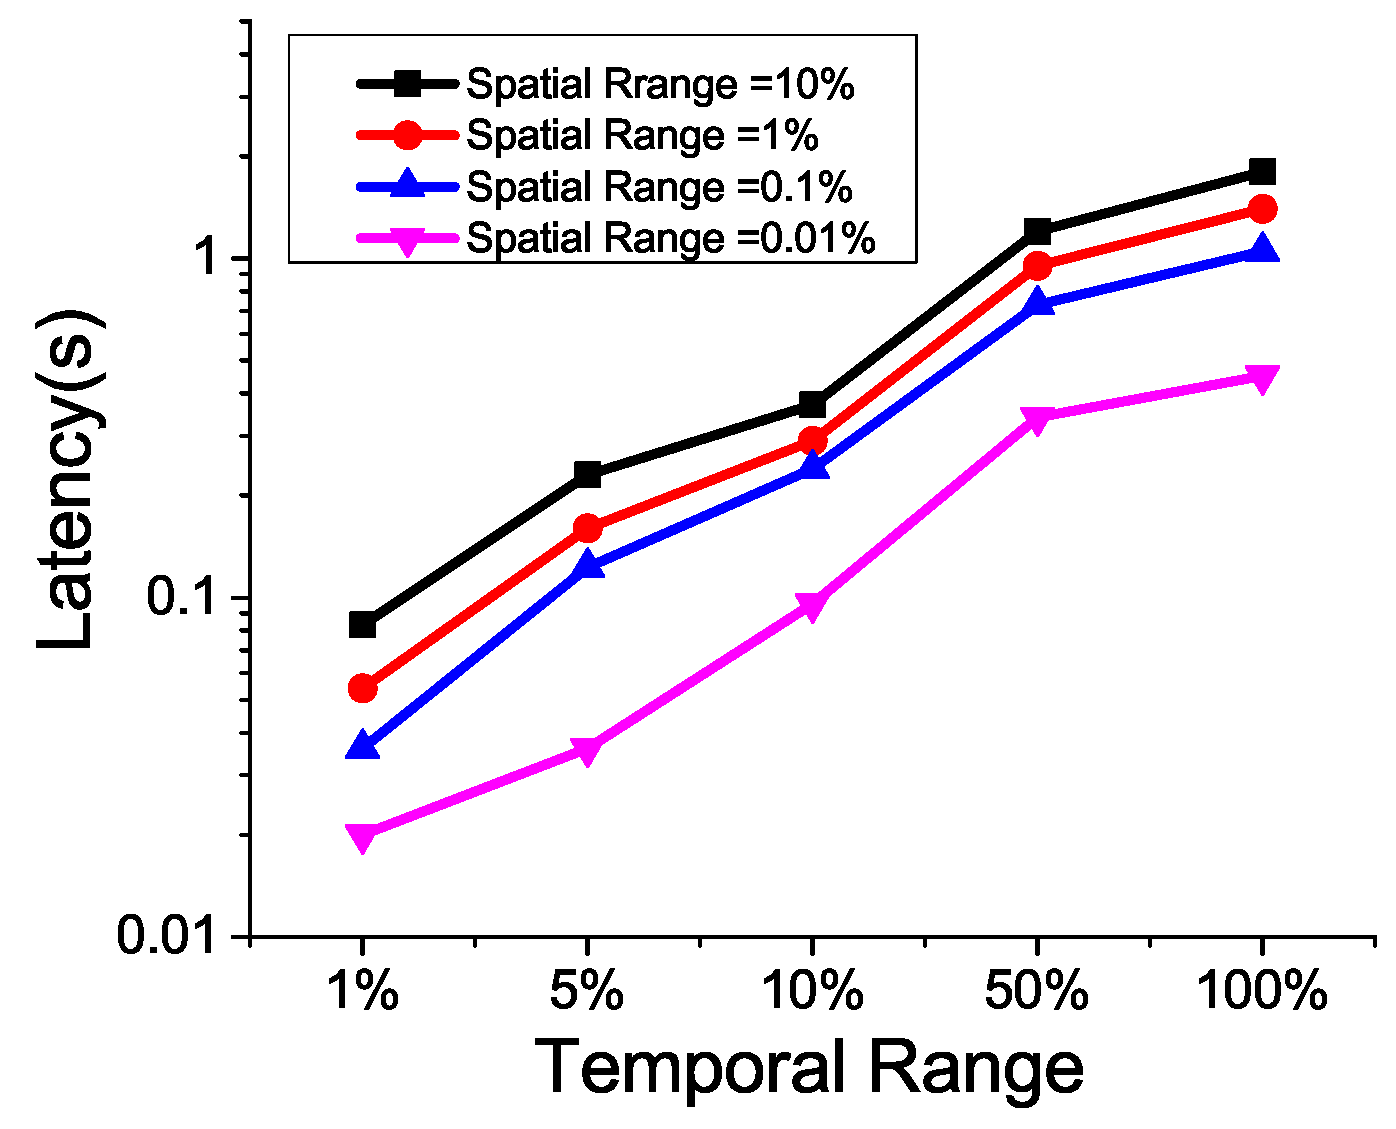
\includegraphics[width=2.7in]{Fig/chapter3/spvSmall.eps}
	}
	\subfigure[TrajSpark---人工数据集]
	{
		\label{fig:GeneratedSPVarious}
		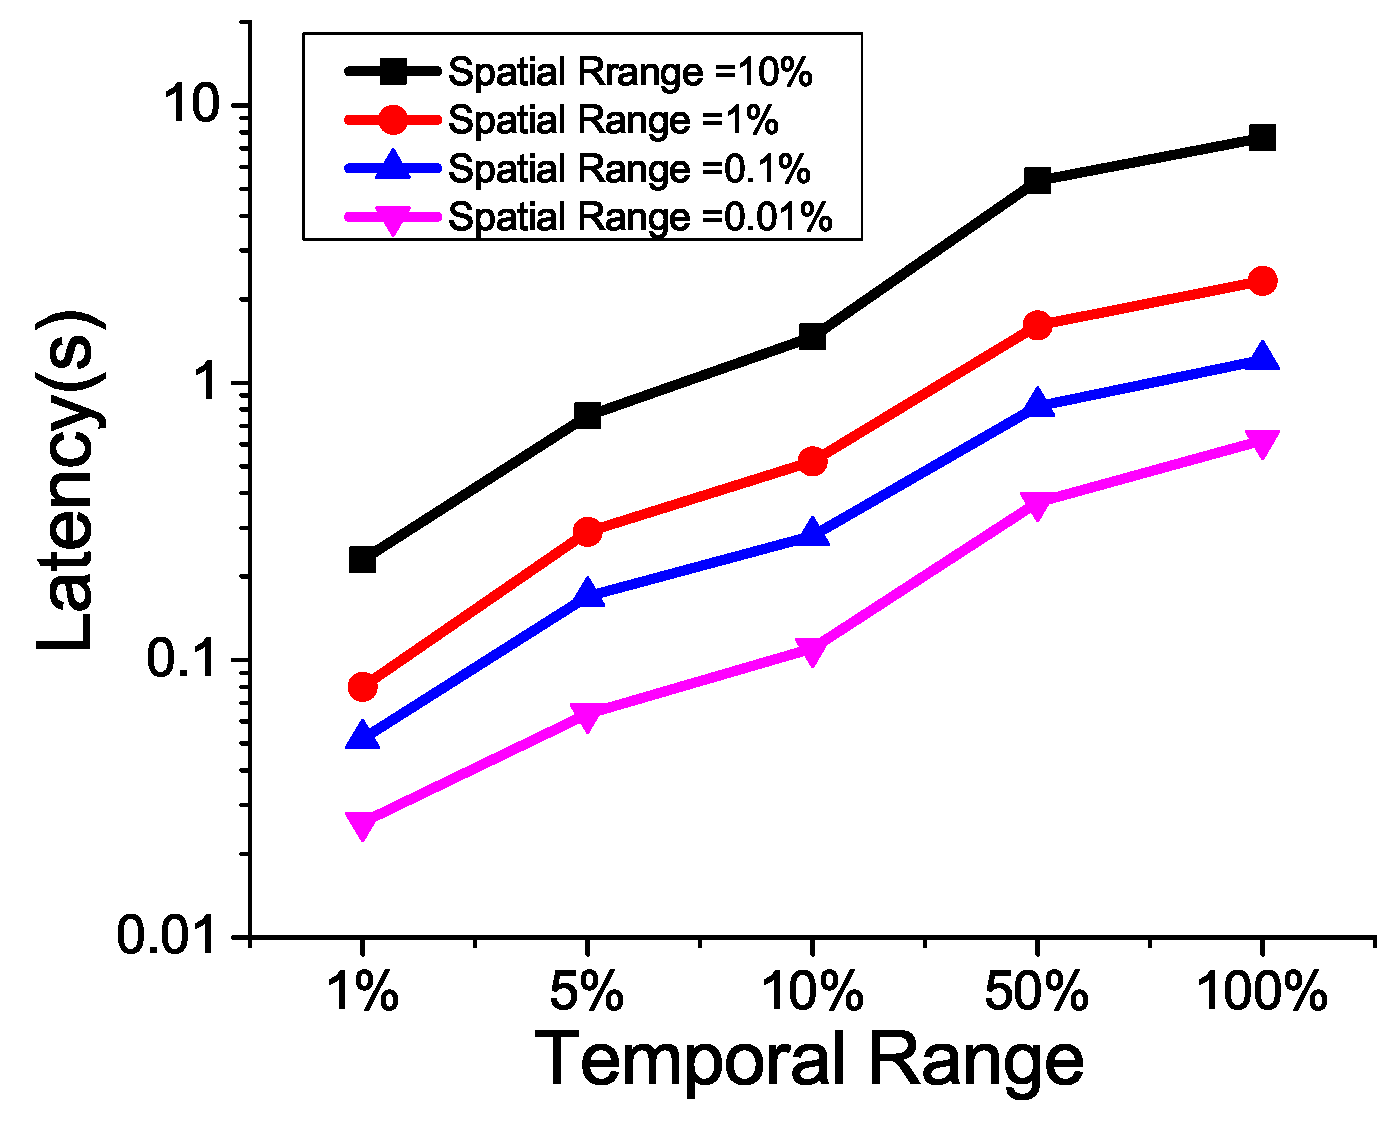
\includegraphics[width=2.7in]{Fig/chapter3/spvBig.eps}
	}
	\caption{时空范围查询性能}
	\label{fig:ST-based}
\end{figure}


\begin{figure}[t]
	\centering
	\subfigure[真实数据集]{  
		\label{fig:knSmallSc}
		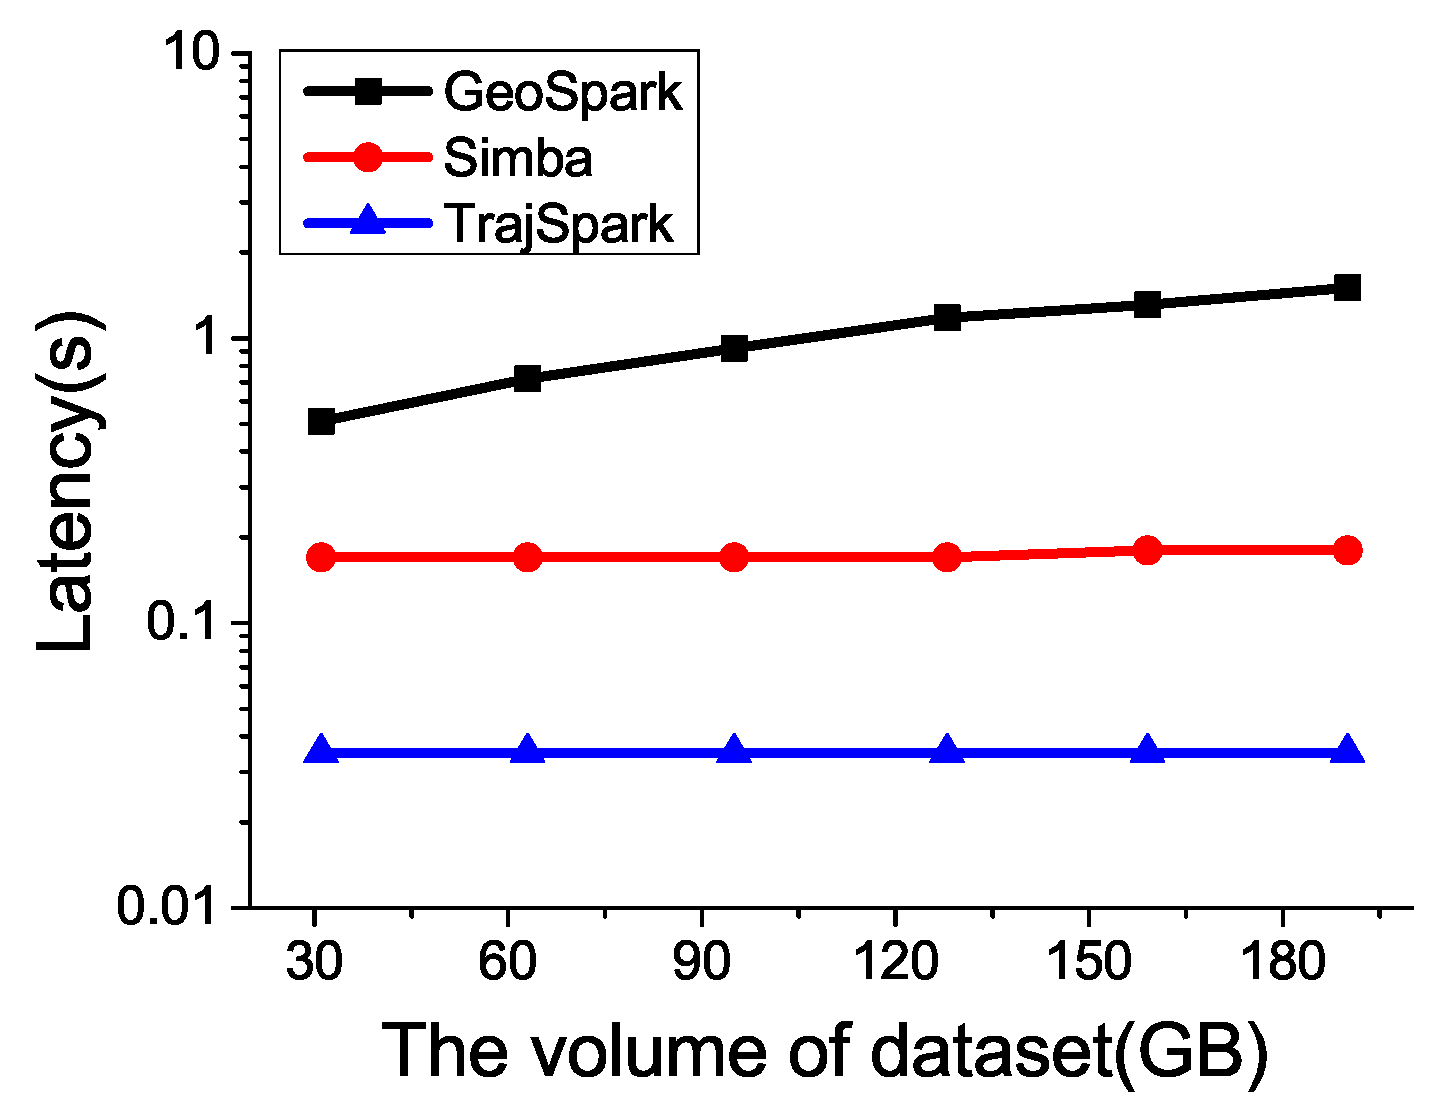
\includegraphics[width=2.7in]{Fig/chapter3/scKNNsmall.eps}	
	}
	\subfigure[人工数据集]{
		\label{fig:knBigSc}
		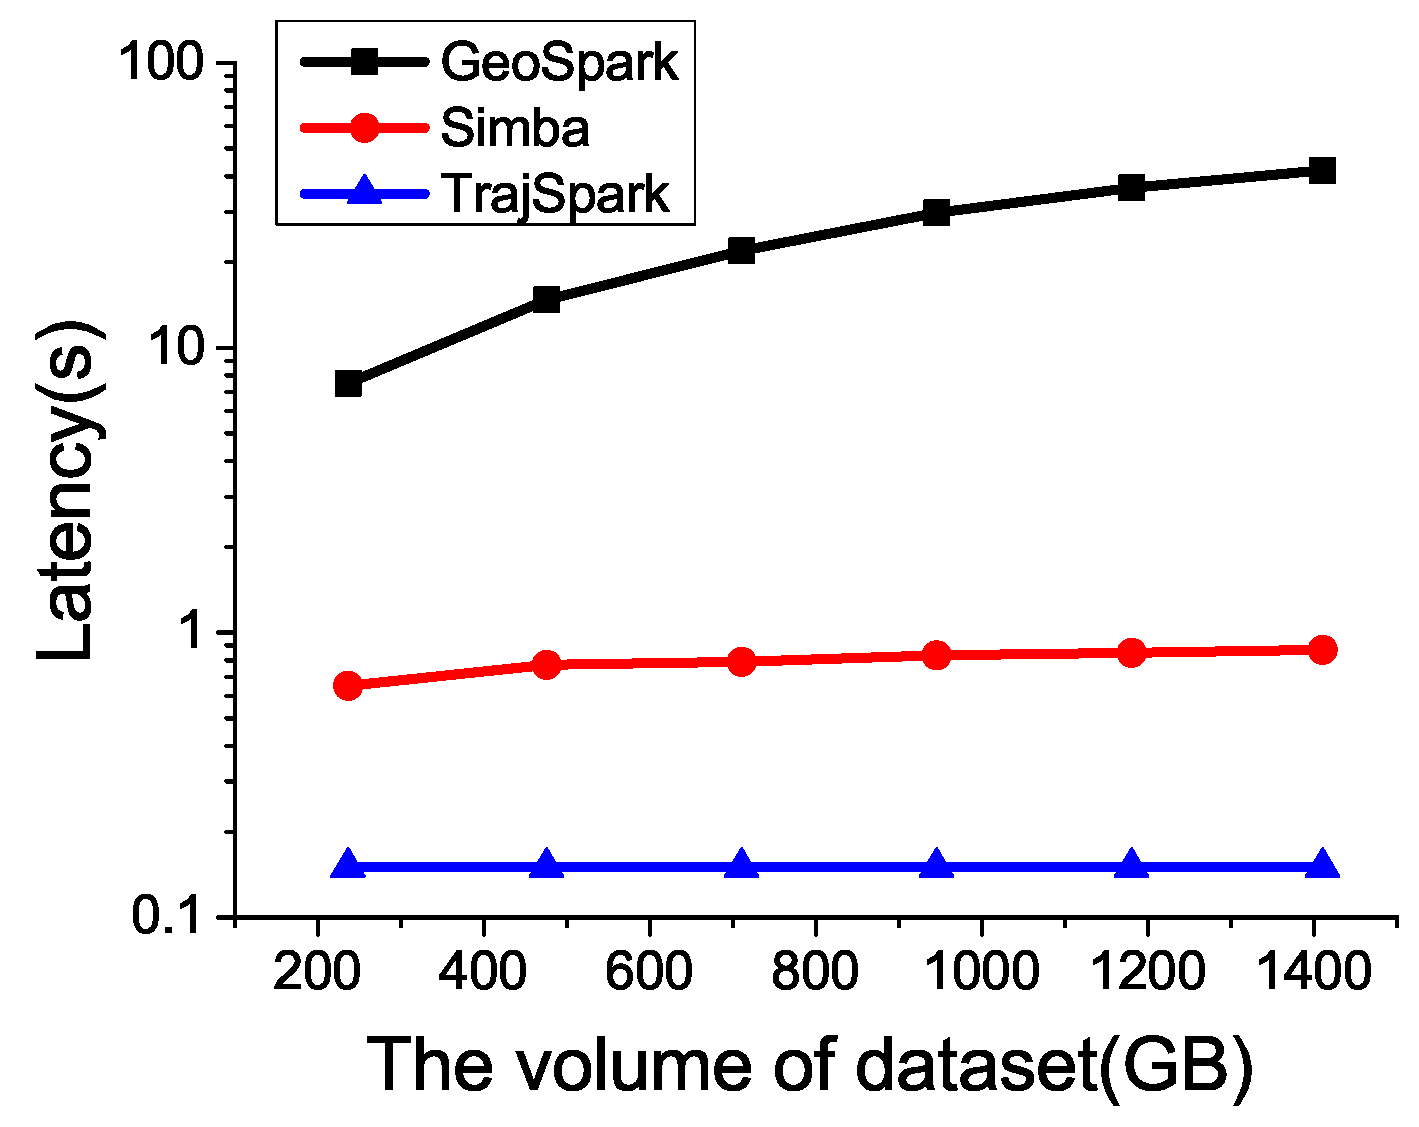
\includegraphics[width=2.7in]{Fig/chapter3/scKNNlarge.eps}
	}\\
	\subfigure[TrajSpark真实数据集]
	{  \label{fig:knSmall}
		\includegraphics[width=2.7in]{Fig/chapter3/knnSmall.eps}
	}
	\subfigure[TrajSpark人工数据集]
	{
		\label{fig:knBig}
		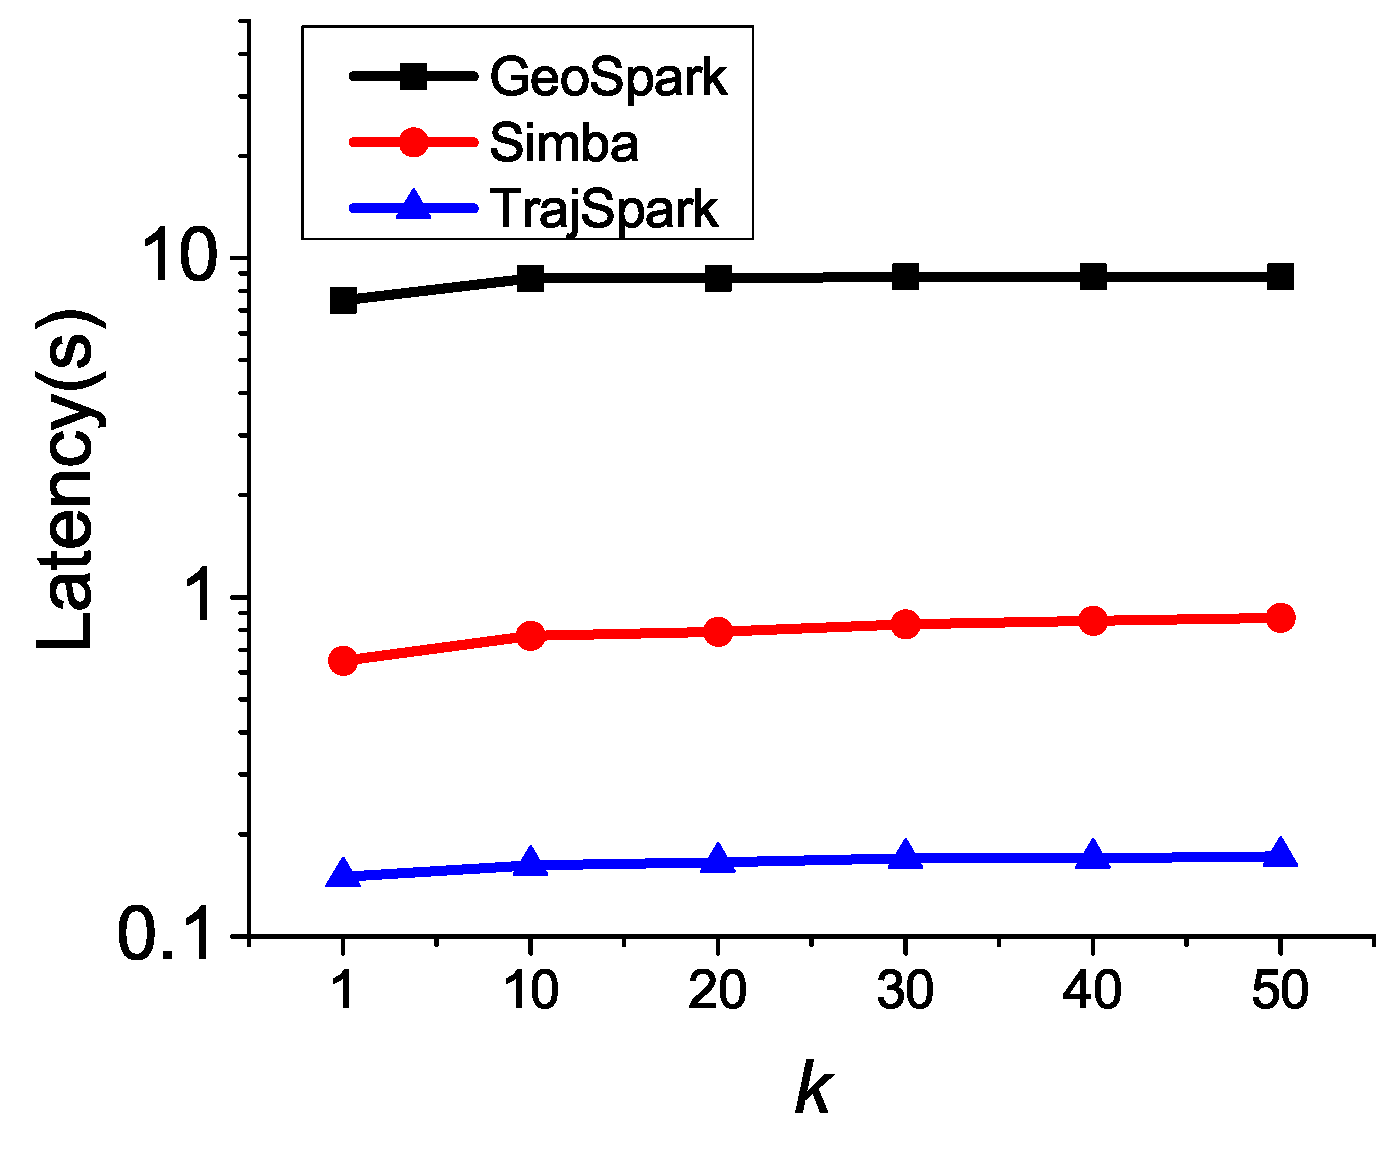
\includegraphics[width=2.7in]{Fig/chapter3/knnLarge.eps}
	}
	\caption{$k$近邻轨迹查询性能}
	\label{fig:knn}
\end{figure}

其次,我们验证了TrajSpark在时空范围下的查询性能。由于数据分布的不均匀性,查询空间范围的选取对查询效率有着较高的影响。为此,我们随机选择了100个包含20*20个方格的区域作为查询的空间约束,选取最近的一周作为当前数据的查询时间约束。查询延时使用100个查询时间的平均值来计算。
实验结果如图\ref{fig:ST-based}所示,其中图\ref{fig:RealST}和\ref{fig:syntheticST}介绍了查询时间随数据量大小的变化情况。我们可以发现,随着数据量的增加,TrajSpark和Simba上的查询效率并没有发生较大变化,这是由于其全局和局部两层索引剪枝的效果。而GeoSpark由于需要遍历数据集,导致随着数据的增加而查询时延逐渐增大。 此外,可以发现 TrajSpark比Simba快了3-5倍,这是由于其可以使用轨迹的MBR和时间范围来快速剪枝轨迹。
此外,我们验证了查询时间随空间和时间约束变化的情况。我们将空间范围选取了整个空间的 $10\%$, $1\%$, 和 $0.1\%$ ,时间范围选取了三个月的后 $100\%$, $50\%$, $10\%$, $5\%$ 和 $1\%$ 。
从图\ref{fig:RealSPVarious}和\ref{fig:GeneratedSPVarious}可以发现随着查询时间和空间范围的增加,查询的时间也随之增加。但增加的方式并不是线性的。比如,当空间范围设置为$0.01\%$时,我们变换时间范围从$1\%$变化 到 $100\%$,空间范围扩大了100倍,但查询时间只延长了30倍。因此,
TrajSpark处理大的时空范围查询仍能取得较好的效果。

再接着,我们验证了TrajSpark处理欧氏距离下$k$近邻查询的性能。
图\ref{fig:knSmallSc} 和\ref{fig:knBigSc} 展示了当 $k$设置为10时,查询时间随数据量大小的变化情况。我们可以发现TrajSpark比GeoSpark快了两个数量级,比Simba快了4-6倍。这是由于TrajSpark和Simba使用全局索引剪枝时空不相关数据分区,而GeoSpark需要遍历数据集的结果。此外TrajSpark由于不需要对同一个移动对象的轨迹点重新排序,因而查询效率更高。这一查询结果与时空范围类似,这是因为$k$近邻查询首先会执行一个迭代的时空范围查询。进一步地,我们将 $k$值从1变化到$50$以查看$k$值对查询效率的影响。从图\ref{fig:knSmall}和\ref{fig:knBig}可以看出$k$值对查询结果影响不大。这是距离较近的轨迹大都放在跟查询轨迹相同的分区内,而每个分区存放的轨迹数远超50个。

 \begin{figure}
	\centering
	\subfigure[]
	{  \label{fig:joinCmp}
		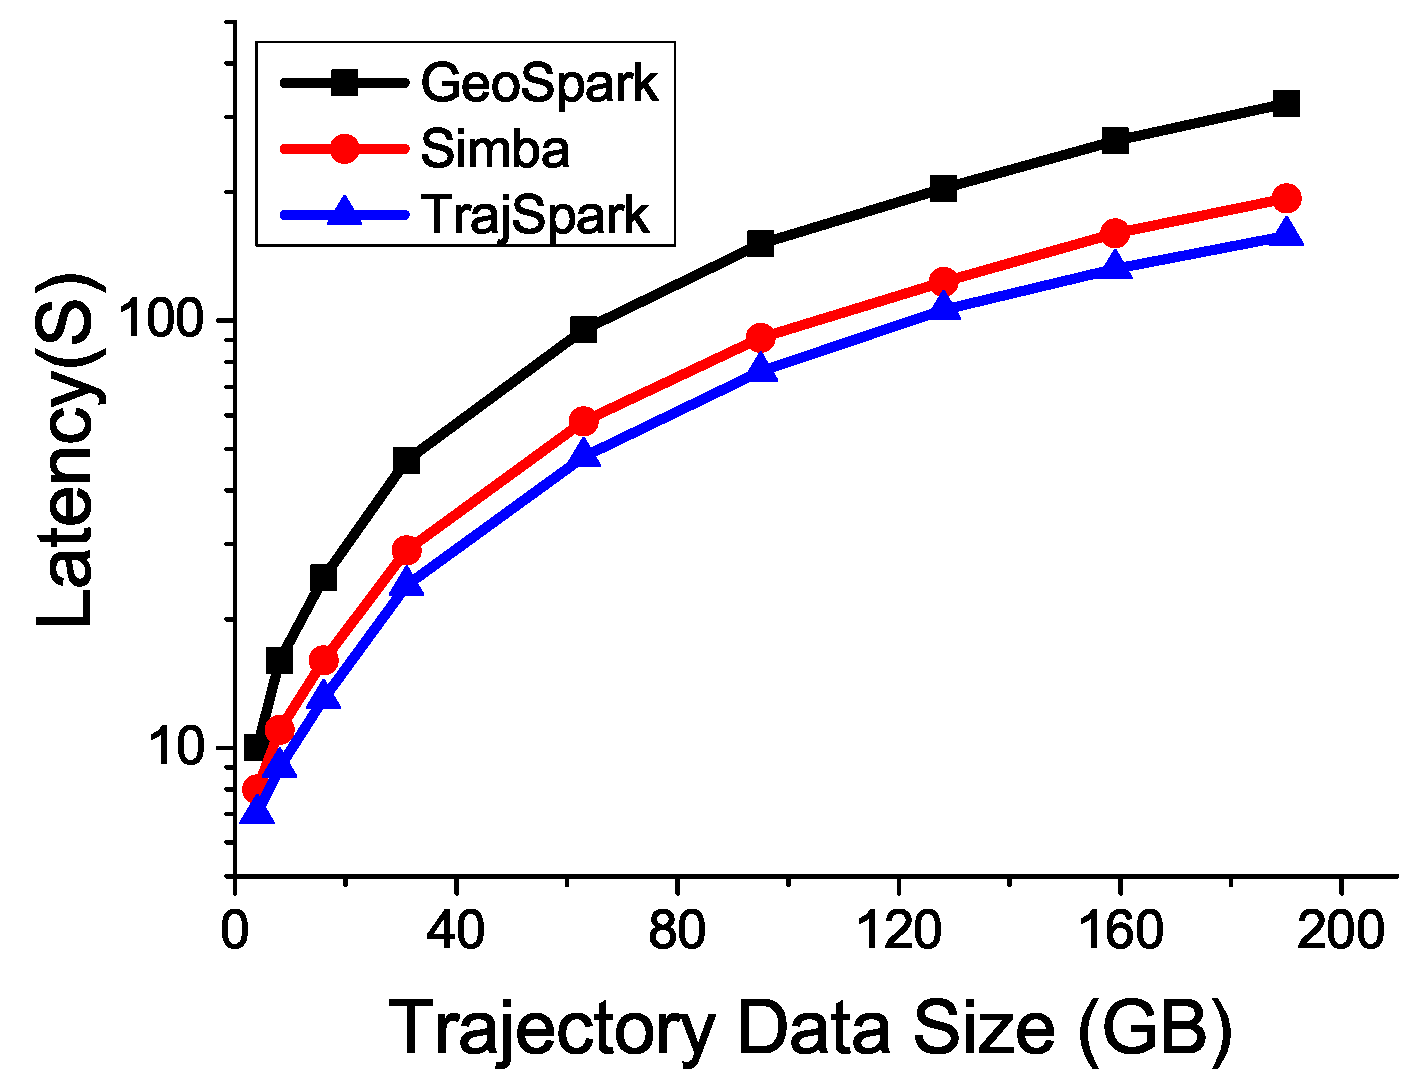
\includegraphics[width=2.7in]{Fig/chapter3/joinCmp.eps}
	}
	%	\hspace{0.005in}
	\subfigure[]
	{
		\label{fig:joinTheta}
		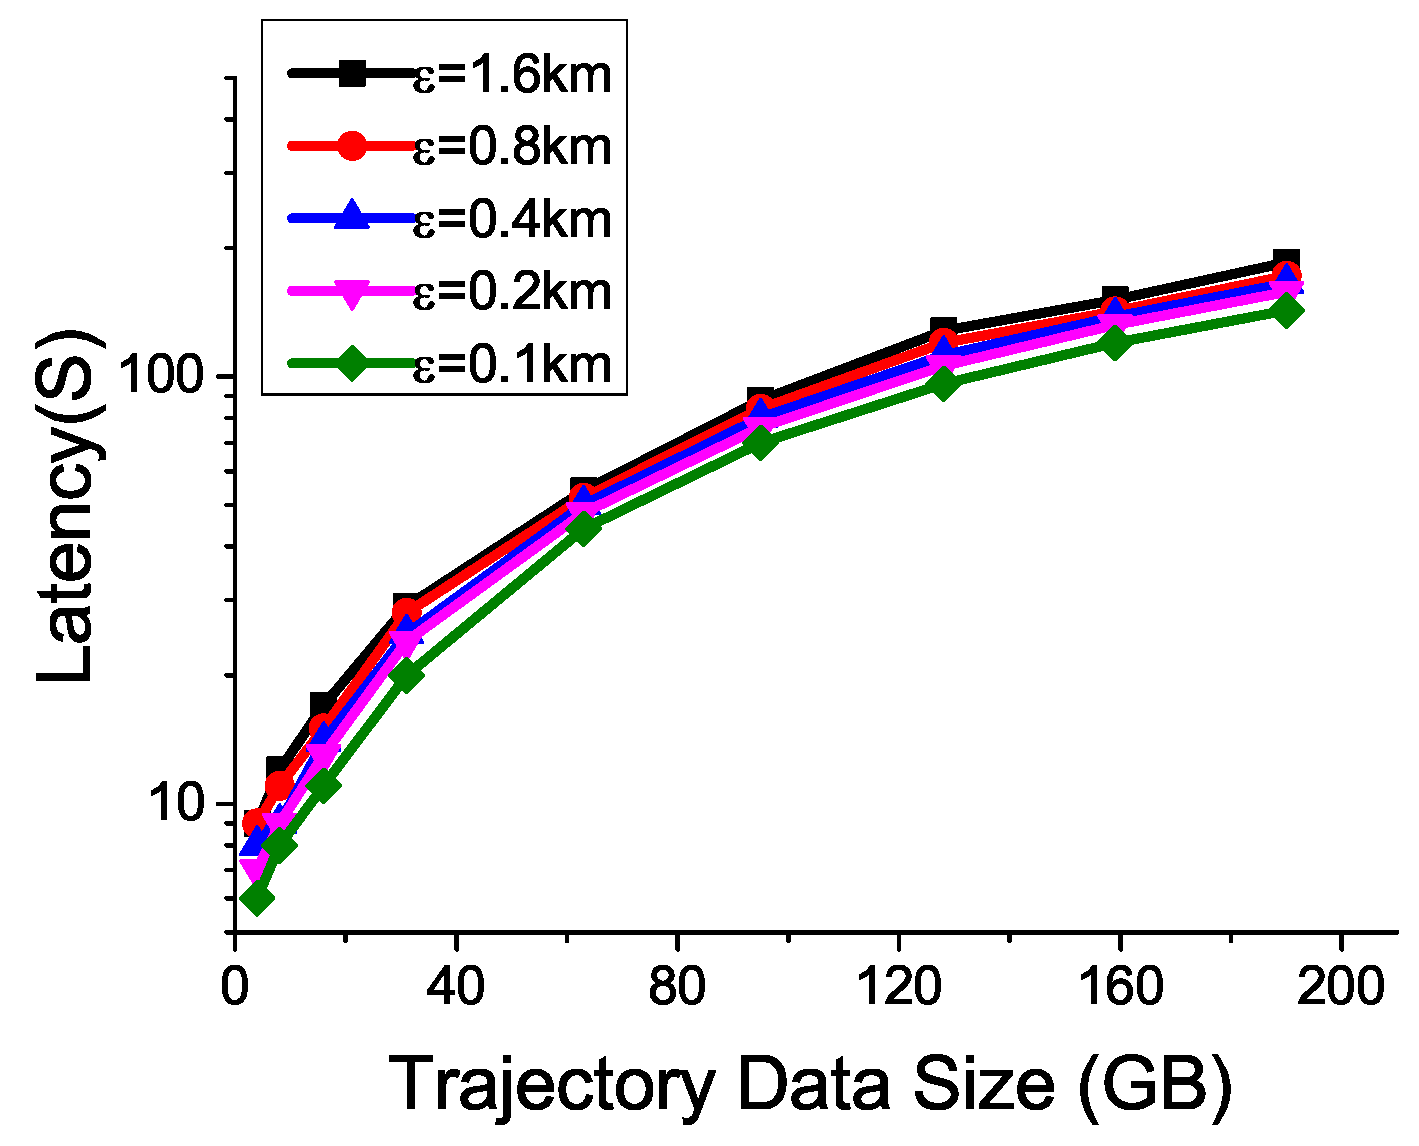
\includegraphics[width=2.7in]{Fig/chapter3/joinTheta.eps}
	}
	\caption{Join查询性能}
	\label{fig:joinExp}
\end{figure}

最后,我们验证了TrajSpark处理join查询的性能。实验所用空间数据集包含两部分数据:北京路网数据结合\cite{ShangZTCY14}和北京POI 数据集合\cite{ShangZTCY14}。其中路网上界集包含148,110  个点 和 196,307条边,而POI数据集包含 273,165 个POI点。
为保持结果简洁,我们只展示了当使用四叉树来索引空间数据的情况(其他索引下结果趋势相同)。Simba实现本文join查询需要结合其自身提供的$k$近邻join和距离约束join两种接口。
Fig. \ref{fig:joinExp}展示了join查询的性能与数据量之间的关系。我们可以发现随着数据量的线性增加,查询时间也呈线性增加。
进一步地,图\ref{fig:joinCmp}对比了当$\epsilon$设置为0.2km 时,不同系统间的性能比较。
这三个系统都支持对轨迹点通过查找空间对象数据集的局部索引以便能快速找到满足 $\epsilon$约束的点,所以都能取得较好的查询结果。
但TrajSpark和Simba比GeoSpark具有更好的加速比,这是因为前两者能通过全局索引,能够剪枝掉不必要的分区对。而GeoSpark由于缺乏全局索引,故需要对其每个SRRD分区匹配空间数据集的每个分区,造成过多不必要的匹配开销。而TrajSpark比Simba性能好的原因是,其对匹配完后的轨迹点无需排序,而Simba是以点的形式管理数据,为形成结果轨迹,需要对属于同一移动对象的点排序。最后,我们验证了算法性能与$\epsilon$的关系。显然地,$\epsilon$值越大,则意味着轨迹点搜索最近邻点的空间越大,从而需要与更多的候选进行距离计算。所以查询时间随着$\epsilon$的增大而增加。但是,由于使用局部索引来搜索候选,导致$\epsilon$增加后仍能快速找到候选。最终,导致$\epsilon$的增加对查询开销的影响不大。

  
\section{本章小结}\label{sec-c3-conclusion}
本章节介绍了使用分布式集群对轨迹大数据进行有效管理并提供实时查询结果。本章节,首先介绍了分布式内存处理系统Spark的相关知识。接着,介绍了基于Spark轨迹数据管理系统及其上经典查询的设计。TrajSpark基于内存的计算思想并引入了全局和局部两层索引,因此设计的查询具有较低的延时。
通过在海量轨迹数据集进行的实验,表明TrajSpark具有较高的查询效果和可扩展性。

\clearpage
\phantom{s}
\clearpage